\documentclass{assignment}

\usepackage{float}
\usepackage{tikz}
\usepackage{adjustbox}
\usepackage{titlesec}
\usepackage{soul}
\usepackage{csvsimple}

\usepackage{graphicx}
\usepackage{subcaption}
\usetikzlibrary{shapes, arrows}

\usetikzlibrary{calc,patterns,angles,quotes}
\setlength{\parindent}{0pt}

\hypersetup{
pdftitle={ME663 - Computational Fluid Dynamics},
pdfsubject={Report for assignment 1},
pdfauthor={Tommaso Bocchietti}
}

\makeglossaries

\newacronym{cfd}{CFD}{Computational Fluid Dynamics}
\newacronym{uds}{UDS}{Upwind Differencing Scheme}
\newacronym{cds}{CDS}{Central Differencing Scheme}
\newacronym{hybrid}{HYBRID}{Hybrid Scheme}
\newacronym{quick}{QUICK}{Quadratic Upstream Interpolation for Convective Kinematics}
\newacronym{gs}{GS}{Gauss-Seidel Iterative Method}
\newacronym{scgs}{SCGS}{Symmetric Coupled Gauss-Seidel}
\newacronym{sim}{SIMPLE}{Semi-Implicit Method for Pressure Linked Equations}

\begin{document}
\graphicspath{{./img/}}


\title{ME663 - Computational Fluid Dynamics \\ Assignment 1}
\author{Tommaso Bocchietti}
\date{A.Y. 2023/24 - W24}

\maketitle

\begin{figure}[H]
    \centering
    
\includegraphics[width=.9\textwidth]{./pdf/UniversityOfWaterloo_logo_vert_pms}
    \label{fig:University_Of_Waterloo_logo}
\end{figure}

\clearpage
\tableofcontents
\listoffigures
\listoftables
\lstlistoflistings
\printglossary[type=\acronymtype]

\clearpage
\section{Requests}
\label{sec:requests}

A system of two aluminum bars of the same material is shown in the following figure.
The system is subjected to two external loads, $P_x$ and $P_y$, at joint B.
A and C are connected to pinned supports.

\begin{figure}[h]
    \centering
    \begin{tikzpicture}[scale=3]

        \coordinate (A) at (0,0.5);
        \coordinate (B) at (3,0.5);
        \coordinate (Bf) at (3.7,1);
        \coordinate (C) at (3,0);

        % Joint names
        \node at (A) [above, left] {A};
        \node at (B) [below, above] {B};
        \node at (C) [below, left] {C};

        % Initial position
        \draw (A) -- (B) node[midway, below] {$L_1$};
        \draw (C) -- (B) node[midway, left] {$L_2$};

        % Deformed position
        \draw[dashed] (A) -- (Bf)node[midway, above] {$l_1$};
        \draw[dashed] (C) -- (Bf)node[midway, right] {$l_2$};

        % Labels
        \pic [draw, ->, "$\alpha$", angle radius=2cm] {angle = B--A--Bf};
        \pic [draw, <-, "$\beta$", angle radius=0.7cm] {angle = Bf--C--B};

        % Support at the end of Beam 1
        \draw[fill] (0,0.5) circle (0.03);

        % Support at the end of Beam 2
        \draw[fill] (3,0) circle (0.03);

        % Arrows at coordinate Bf
        \draw[->] (Bf) -- ++(0.3, 0) node[right] {$\vec{P_x}$};
        \draw[->] (Bf) -- ++(0, 0.3) node[above] {$\vec{P_y}$};
        \draw[->] (B) -- (Bf) node[midway, above] {$\vec{u}$};
        % \draw[->, shorten >=150pt] (Bf) -- (A) node[above, above] {$\vec{F_1}$};
        % \draw[->, shorten >=50pt] (Bf) -- (C) node[above, right] {$\vec{F_2}$};

    \end{tikzpicture}
    \caption{Problem representation}
    \label{fig:problem_representation}
\end{figure}

The problem asks to:

\begin{itemize}
    \item Obtain the external loads $P_x$ and $P_y$ as a function of horizontal and vertical displacements at point B (namely $u$ and $v$).
    \item Determine the displacements in both $x$ and $y$ directions for $1000$ load increments of $+5\text{N}$ for both $P_x$ and $P_y$ (from zero).
    \item Find the displacement of point B after the final increment.
\end{itemize}

Write a \texttt{MATLAB} code with a convergence error of $10^-5$ to numerically solve the problem.
Use a combination of (a) Euler and N-R, and (b) Euler and modified N-R.
Also plot the resultant force versus the resultant displacement.

Use the Green strain measure:

\begin{equation}
    E_i = \frac{l_i^2 - L^2}{2L^2}
    \label{eq:green_strain_measure_formula}
\end{equation}

From now on, we will refer to the Green strain measure as $\epsilon_{1,2}$ to differentiate it from the Young's modulus $E_{1,2}$.

\begin{table}[H]
    \centering
    \begin{tabular}{|c|c|c|}
        \hline
        \textbf{Parameter} & \textbf{Value} & \textbf{Unit} \\ \hline
        $E_1 = E_2 = E$    & $70$           & $\text{GPa}$  \\ \hline
        $L_1$              & $3$            & $\text{m}$    \\ \hline
        $L_2$              & $0.5$          & $\text{m}$    \\ \hline
        $A_1 = A_2 = A$    & $0.0001$       & $\text{m}^2$  \\ \hline
    \end{tabular}
    \caption{Parameters of the system}
    \label{tab:parameters_of_the_system}
\end{table}

\section{Methods}
\label{sec:methods}

\paragraph{Research Methodology}
The research will be conducted through a literature review of scientific articles, conference papers and thesis if available.
The main sources of information will be the IEEE Xplore, ScienceDirect, and Google Scholar databases.
The search will be conducted using the following keywords: "Chip-Scale Atomic Clock", "Atomic Clock", "MEMS", "CSAC", "Vapor Cell", "Rubidium", "Cesium", "Microwave Cavity", "Laser Cooling", "Photon Detector", "Quartz Crystal Oscillator", "Electron Spin", "Electron Excitation", "Optical Lattice Clock", "Quantum Technologies".

During the research, we will try to annotate the most relevant papers and articles, that will be then used to write the final report.

\paragraph{Outline}
We leave here a general outline that will be used as a guide for the development of the project.

\begin{enumerate}
    \item Introduction: Discuss the need for precise timekeeping and the exigence of chip-scale atomic clocks.
    \item \textbf{Engineering of Chip-Scale Atomic Clocks}: Discuss the principles of operation. Note: It would be interesting to use simulation tools such as \texttt{COMSOL Multiphysics} to visualize the operating principles of these devices, but not knowing the software and its capabilities, I am not sure if it is applicable here.
          \begin{itemize}
              \item Vapour cell
              \item Magnetic selector (electron spin)
              \item Microwave cavity (electron excitation at hyperfine transition)
              \item Laser system (laser cooling and trapping of atoms)
              \item Photon detector
              \item Closed loop over quartz crystal oscillator
          \end{itemize}
          \begin{figure}[H]
              \centering
              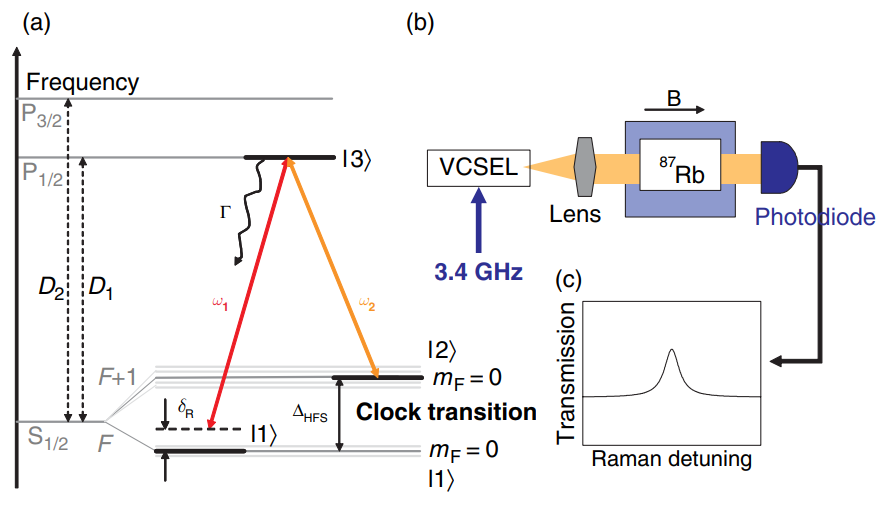
\includegraphics[width=.6\textwidth]{img/atomic_clock_logic}
              \caption{Schematic of the simplified atomic energy level configuration \cite{KNAPPE2008571}}
          \end{figure}

    \item \textbf{Technology Comparison}: Introduce the different types of chip-scale atomic clocks. Compare and contrast the different chip-scale atomic clock technologies in terms of size, power consumption, accuracy, and suitability for various applications.
          \begin{itemize}
              \item Cesium based
              \item Rubidium based
          \end{itemize}
          % \item Fabrication and Manufacturing: Explore the components of chip-scale atomic clocks such as atomic vapor cells, laser systems, and control electronics. Understand the microfabrication techniques used in their manufacturing.
    \item Applications: Consider the diverse applications of chip-scale atomic clocks (aerospace and defense to telecommunications and scientific research)
    \item Challenges and Future Directions: Identify current challenges such as size reduction and power efficiency, and consider future trends like adoption of optical lattice clocks and integration with quantum technologies.
    \item Conclusion: Summarize the key findings of the research and discuss the implications for future advancements and applications of chip-scale atomic clocks.
\end{enumerate}

% In case of time availability, we will also cover the Fabrication and Manufacturing of these devices, understanding the microfabrication techniques used in their manufacturing.

\paragraph{Time schedule}
In general, given a time constraint of 4/5 weeks, the project will be divided as follows (tentative)

\begin{itemize}
    \item Week 1: Introduction + Engineering of Chip-Scale Atomic Clocks
    \item Week 2: Engineering of Chip-Scale Atomic Clocks (possible simulation and results analysis)
    \item Week 3: Technology Comparison + Applications
    \item Week 4: Challenges and Future Directions + Conclusion
    \item Week 5: Final report writing
\end{itemize}

\section{Derivation of discretized governing equations}
\label{sec:derivation_of_discretized_governing_equations}

In this section, we will derive the discretized governing equations for the incompressible Navier-Stokes equations, which will be used to solve the problem at hand.

The set of incompressible Navier-Stokes equations is given by:

\begin{equation*}
    \nabla \cdot {\mathbf{u}} = 0
    \label{eq:incompressible_navier_stokes_continuity}
\end{equation*}

\begin{equation*}
    \rho \frac{\partial \mathbf{u}}{\partial t} + \rho \mathbf{u} \cdot \nabla \mathbf{u} = -\nabla p + \mu \nabla^2 \mathbf{u} + \mathbf{f}
    \label{eq:incompressible_navier_stokes_momentum}
\end{equation*}

In the rest of the document, the following hypotheses will be considered:

\begin{itemize}
    \item Steady-state problem: $\frac{\partial \mathbf{u}}{\partial t} = 0$
    \item Constant density: $\rho = \text{const}$
    \item Constant dynamic viscosity: $\mu = \text{const}$
    \item Zero body forces: $\mathbf{f} = 0$
\end{itemize}

Based on these hypotheses, the incompressible Navier-Stokes equations can be simplified and expanded as follows:

\begin{align}
    \frac{\partial u}{\partial x} + \frac{\partial v}{\partial y}     & = 0                                                                                                                         \\
    \frac{\partial u u}{\partial x} + \frac{\partial v u}{\partial y} & = -\frac{\partial p}{\partial x} + \nu \left( \frac{\partial^2 u}{\partial x^2} + \frac{\partial^2 u}{\partial y^2} \right) \\
    \frac{\partial u v}{\partial x} + \frac{\partial v v}{\partial y} & = -\frac{\partial p}{\partial y} + \nu \left( \frac{\partial^2 v}{\partial x^2} + \frac{\partial^2 v}{\partial y^2} \right)
    \label{eq:incompressible_navier_stokes_steady_2D}
\end{align}

Where $\nu = \frac{\mu}{\rho}$ is the kinematic viscosity and $p = \frac{p}{\rho}$ is the non-dimensional pressure.

Obviously, to solve the problem using a discrete calculator, the equations must be therefore discretized.

\subsection{Finite Volume Method}
\label{subsec:finite_volume_method}

The Finite Volume Method (FVM) is a numerical technique used to discretize partial differential equations, and is particularly well suited for the discretization of the Navier-Stokes equations.

The idea here is to divide the domain into a set of control volumes, and then integrate the governing equations over each control volume.
The resulting set of equations will be a set of algebraic equations, which can be solved using a discrete calculator.


\subsubsection{Control volumes}

Before proceeding with the discretization of the governing equations, we need to define what a control volume is and the notations used in the rest of the document.

In particular, we will assume from now on to have a Cartesian grid, with a uniform mesh spacing in both the $x$ and $y$ directions.

From the Figure \ref{fig:control_volume}, we can appreciate graphically how the domain is divided.

\begin{figure}[H]
    \centering
    \def\nCV{5}
    \def\dX{1.5cm}
    \def\dY{1.5cm}
    \def\labelsH{{"WW", "W", "P", "E", "EE"}}
    \def\labelsV{{"SS", "S", "P", "N", "NN"}}

    \begin{tikzpicture}

        \foreach \n in {0,1,...,\nCV}
            {
                \draw (0, \n*\dY) -- (\nCV*\dX, \n*\dY);
                \draw (\n*\dX, 0) -- (\n*\dX, \nCV*\dY);
            }

        % \foreach \n in {0,1,...,\the\numexpr\nCV-1\relax}
        %     {
        %         \draw[dashed] (-\dX/2, \n*\dY + \dY/2) -- (\nCV*\dX+\dX/2, \n*\dY + \dY/2);
        %         \draw[dashed] (\n*\dX + \dX/2, -\dY/2) -- (\n*\dX + \dX/2, \nCV*\dY+\dY/2);
        %     }

        \foreach \y in {0,1,...,\the\numexpr\nCV-1\relax}
            {
                \foreach \x in {0,1,...,\the\numexpr\nCV-1\relax}
                    {
                        \node[font=\small] at (\x*\dX+\dX/6, \y*\dY+\dY/10) {$_{\the\numexpr\x+1\relax,\the\numexpr\y+1\relax}$};
                    }
            }

        \foreach \n in {0,1,...,\the\numexpr\nCV-1\relax}
            {
                \node[font=\small] at (\n*\dX+\dX/2, \nCV/2*\dY) {\pgfmathparse{\labelsH[\n]}\pgfmathresult};
                \node[font=\small] at (\nCV/2*\dX, \n*\dY+\dY/2) {\pgfmathparse{\labelsV[\n]}\pgfmathresult};
            }

        \node[font=\small] at (\nCV/2*\dX, \nCV/2*\dY+\dY/2) {$s$};
        \node[font=\small] at (\nCV/2*\dX, \nCV/2*\dY-\dY/2) {$n$};
        \node[font=\small] at (\nCV/2*\dX-\dX/2, \nCV/2*\dY) {$w$};
        \node[font=\small] at (\nCV/2*\dX+\dX/2, \nCV/2*\dY) {$e$};

        \fill[yellow, opacity=0.3] (\nCV/2*\dX-\dX/2, \nCV/2*\dY-\dY/2) rectangle (\nCV/2*\dX+\dX/2, \nCV/2*\dY+\dY/2);

    \end{tikzpicture}
    \caption{Control volumes and control volume faces.}
    \label{fig:control_volume}
\end{figure}

In particular, Figure \ref{fig:control_volume} shows:

\begin{itemize}
    \item A grid of control volumes, with the subscript $(i,j)$ indicating the position of the control volume in the $x$ and $y$ directions, respectively. For example, the control volume in the center of the grid has indices $(i,j)=(3,3)$.
    \item The control volume centers with capital letters, $P, N, S, E, W, \ldots$.
    \item The control volume faces with lowercase letters, $n, s, e, w$.
\end{itemize}

Notice also that the capital letters always refers to a relative position with respect to the control volume in consideration.
For example, $P$ refers to the control volume in consideration, $N$ refers to the control volume to the north of $P$, and so on.
For this reason, in Figure \ref{fig:control_volume}, the control volume $P$ is highlighted in yellow so to indicate that is the control volume in consideration.


\subsubsection{Staggered grid and $L_{shape}$}

As we will see later during the formulation of the solving solution, for the purpose of this work, we will use a specific type of grid, called staggered grid.

We can also give a brief definition of the two types of grids available in the literature, which are:

\begin{itemize}
    \item \textbf{Collocated grid}: all the variables are located at the same point in the control volume (e.g. the center of the control volume).
    \item \textbf{Staggered grid}: the variables are located at different points in the control volume (e.g. the velocity components are located at the center of the faces of the control volume, and the pressure is located at the center of the control volume).
\end{itemize}

Given the formulation of the staggered grid, it's now useful to define the so called $L_{shape}$, which is a frame used to define in a compact and clear way the position of the variables in the control volume.

The $L_{shape}$ has been reported for control volume $P$ in Figure \ref{fig:L_shape}.

\begin{figure}[H]
    \centering
    \def\nCV{3}
    \def\dX{3cm}
    \def\dY{3cm}
    \def\labelsH{{"W", "P", "E"}}
    \def\labelsV{{"S", "P", "N"}}

    \begin{tikzpicture}

        \foreach \n in {0,1,...,\nCV}
            {
                \draw (0, \n*\dY) -- (\nCV*\dX, \n*\dY);
                \draw (\n*\dX, 0) -- (\n*\dX, \nCV*\dY);
            }

        \foreach \n in {0,1,...,\the\numexpr\nCV-1\relax}
            {
                \draw[dashed] (-\dX/2, \n*\dY + \dY/2) -- (\nCV*\dX+\dX/2, \n*\dY + \dY/2);
                \draw[dashed] (\n*\dX + \dX/2, -\dY/2) -- (\n*\dX + \dX/2, \nCV*\dY+\dY/2);
            }

        \foreach \y in {0,1,...,\the\numexpr\nCV-1\relax}
            {
                \foreach \x in {0,1,...,\the\numexpr\nCV-1\relax}
                    {
                        \node[font=\small] at (\x*\dX+\dX/10, \y*\dY+\dY/15) {$_{\the\numexpr\x-(\nCV-1)/2\relax,\the\numexpr\y-(\nCV-1)/2\relax}$};
                    }
            }

        \foreach \n in {0,1,...,\the\numexpr\nCV-1\relax}
            {
                \node[font=\small] at (\n*\dX+\dX/2, \nCV/2*\dY) {\pgfmathparse{\labelsH[\n]}\pgfmathresult};
                \node[font=\small] at (\nCV/2*\dX, \n*\dY+\dY/2) {\pgfmathparse{\labelsV[\n]}\pgfmathresult};
            }

        \draw[thick, blue, ->] (\nCV/2*\dX, \nCV/2*\dY)++(0,  \dY/4) -- ++(0, \dY/2) node[pos=1, right] {$u_s$};
        \draw[thick, blue, ->] (\nCV/2*\dX, \nCV/2*\dY)++(0, -\dY/2-\dY/4) -- ++(0, \dY/2) node[pos=1, right] {$u_s$};
        \draw[thick, red, ->] (\nCV/2*\dX, \nCV/2*\dY)++(\dX/4, 0) -- ++(\dX/2, 0) node[pos=1, above] {$u_e$};
        \draw[thick, red, ->] (\nCV/2*\dX, \nCV/2*\dY)++(-\dX/2-\dX/4, 0) -- ++(\dX/2, 0) node[pos=1, above] {$u_w$};

        \fill[yellow, opacity=0.3] (\nCV/2*\dX-\dX/2, \nCV/2*\dY-\dY/2) rectangle (\nCV/2*\dX+\dX/2, \nCV/2*\dY+\dY/2);

    \end{tikzpicture}
    \caption{$L_{shape}$ for control volume $P$.}
    \label{fig:L_shape}
\end{figure}

Basically, the $L_{shape}$ for control volume $P$ links the velocity components to the control volume $P$ itself, and it's used to define the indexes of the system.

In particular, the same Figure \ref{fig:L_shape} can be represented using the index notations, as shown in Figure \ref{fig:L_shape_index}.

\begin{figure}[H]
    \centering
    \def\nCV{1}
    \def\dX{5cm}
    \def\dY{5cm}

    \begin{tikzpicture}[every node/.style={font=\huge}]

        \draw (0, 0) -- (\dX, 0) -- (\dX, \dY) -- (0, \dY) -- cycle;

        \node at (\dX/7, \dY/10) {$i,j$};

        \node at (\dX/2, \dY/2) {$P_{i,j}$};

        \draw[thick, blue, ->] (\dX/2, \dY/2)++(0,  \dY/4) -- ++(0, \dY/2) node[pos=1, right] {$u_{i,j}$};
        \draw[thick, blue, ->] (\dX/2, \dY/2)++(0, -\dY/2-\dY/4) -- ++(0, \dY/2) node[pos=1, right] {$u_{i,j-1}$};
        \draw[thick, red, ->] (\dX/2, \dY/2)++(\dX/4, 0) -- ++(\dX/2, 0) node[pos=1, above] {$u_{i,j}$};
        \draw[thick, red, ->] (\dX/2, \dY/2)++(-\dX/2-\dX/4, 0) -- ++(\dX/2, 0) node[pos=1, above] {$u_{i-1,j}$};

        \draw[yellow,
            opacity=0.3,
            line cap=round,
            double=yellow,
            double distance=\dX/5,
        ] (\dX/2, \dY/2) -- ++(0, \dY/2+\dY/4);

        \draw[yellow,
            opacity=0.3,
            line cap=round,
            double=yellow,
            double distance=\dX/5,
        ] (\dX/2, \dY/2) -- ++(\dX/2+\dX/4, 0);

        \draw[dashed, |-|] (0, -\dY/6) -- (\dX, -\dY/6) node[pos=1, below, font=\Large] {$\Delta x$};
        \draw[dashed, |-|] (-\dX/6, 0) -- (-\dX/6, \dY) node[pos=1, left, font=\Large] {$\Delta y$};

    \end{tikzpicture}
    \caption{$L_{shape}$ for control volume $P$ using index notations.}
    \label{fig:L_shape_index}
\end{figure}

From Figure \ref{fig:L_shape_index}, we can appreciate how the $L_{shape}$ works well with index notations, and can be useful when working purely with indexes to refer to the variables.
\subsection{Application of the Finite Volume Method}
\label{subsec:application_of_the_finite_volume_method}

Having defined our working framework, we can now proceed to the application of the Finite Volume Method (FVM) to the incompressible Navier-Stokes equations \ref{eq:incompressible_navier_stokes_steady_2D}.

To do so, we start by giving the general integral form of the governing equations, and then proceed to the discretization of the convection, diffusion and source terms separately.

In particular, assuming from now on to have a Cartesian grid, with a uniform mesh spacing in both the $x$ and $y$ directions, the (FVM) reads as follows:




From now on, we will focus on the $x$ direction, given that the treatment for the $y$ direction is analogous.

The first step is to integrate the governing equations over each control volume.

Our discretized set of equations will be:

\begin{align}
    % TODO Check if the equation is correct
    \int_{V} u \frac{\partial u}{\partial x} dV + v \frac{\partial u}{\partial y} dV - \frac{1}{\rho} \frac{\partial p}{\partial x} dV - \nu \left( \frac{\partial^2 u}{\partial x^2} + \frac{\partial^2 u}{\partial y^2} \right) dV - f_x dV = 0 \\
    \int_{V} u \frac{\partial v}{\partial x} dV + v \frac{\partial v}{\partial y} dV - \frac{1}{\rho} \frac{\partial p}{\partial y} dV - \nu \left( \frac{\partial^2 v}{\partial x^2} + \frac{\partial^2 v}{\partial y^2} \right) dV - f_y dV = 0
\end{align}

We can now proceed to the discretization of the convection, diffusion and source terms separately.

The rest of the treatment will be done considering just the $x$ direction, given that the treatment for the $y$ direction is analogous.

Our starter equation is:

\begin{equation}
    \int_{V} \underbrace{u \frac{\partial u}{\partial x} + v \frac{\partial u}{\partial y}}_{\text{Convection term}} - \underbrace{\frac{1}{\rho} \frac{\partial p}{\partial x} dV}_{\text{Pressure term}} - \underbrace{\nu \left( \frac{\partial^2 u}{\partial x^2} + \frac{\partial^2 u}{\partial y^2} \right) dV}_{\text{Diffusion term}} - \underbrace{f_x dV}_{\text{Source term}} = 0
    \label{eq:inc_navier_stokes_steady_2D_discretized_x}
\end{equation}

Before proceeding, we need to define the control volume and the control volume faces geometrically.



% \subsection{Convection term}
\label{subsec:convection_term}
% \subsection{Diffusion term}
\label{subsec:diffusion_term}
% \subsection{Source term}
\label{subsec:source_term}
% \input{src/03.4 - discretized_governing_equations}


\section{Schemes}
\label{sec:schemes}

In this section, we will present the schemes used to solve the previously quasi-discretized equations \ref{eq:INS_steady_2D_discretized_convection} and \ref{eq:INS_steady_2D_discretized_diffusion}.

Those schemes are the "tools" that will allow us to bind the currently considered cell values with its neighbor's cell values.
This means that at the end of this section, we will have a set of coefficients (based on the scheme adopted) that will be used to assemble the solving matrix of the system.

To further clarify, what we want to achieve is to compute the following functions ($nb$ indicates a generic neighbor cell, one or more cells away from the current cell $P$):

\begin{align}
    u_P & = f(u_{nb}, v_{nb}, p_{nb}) \\
    v_P & = f(u_{nb}, v_{nb}, p_{nb})
\end{align}

As we will see, the result of the schemes will be a set of coefficients that will be used to compute the values of $u_P$ and $v_P$ based on the values of the neighbor cells.
In particular, the final form of the system will be:

\begin{align}
    A_P^u u_P & = \sum_{nb} A_{nb}^u u_{nb} + b_P^u \\
    A_P^v v_P & = \sum_{nb} A_{nb}^v v_{nb} + b_P^v
    \label{eq:coefficients_form_system}
\end{align}

Notice how there is no direct correlation between the $u$ and $v$ equations, that are instead coupled through the pressure term $p$.

Using the indices' notation system $(i,j)$ becomes:

\begin{align}
    (A_P^u)_{i,j} u_{i,j} & = \sum_{nb} (A_{nb}^u)_{i,j} u_{i,j} + (p_{i,j} - p_{i+1,j}) \Delta y \\
    (A_P^v)_{i,j} v_{i,j} & = \sum_{nb} (A_{nb}^v)_{i,j} v_{i,j} + (p_{i,j} - p_{i,j+1}) \Delta x
\end{align}

Similar to the approach used in the previous section, we will treat separately the convection and diffusion terms.
In this way we will obtain two different sets of coefficients, one for the convection term and one for the diffusion term.
Those coefficients will be then reassembled together to reduce the equations to the final form presented above.

In particular, we will have that the coefficients $A_P^\phi$ and $A_{nb}^\phi$ will be the difference between the convection and diffusion coefficients, given that from Equation \ref{eq:FVM_momentum_x_direction}, we know:

\begin{equation}
    FVM_{\text{Convection}} - FVM_{\text{Diffusion}} = 0 \rightarrow (A^\phi) = (A^\phi)_{\text{Convection}} - (A^\phi)_{\text{Diffusion}}
\end{equation}

\textbf{Note:} In the following sections, we will refer to the use of \texttt{Mathematica}.
The complete notebook used to obtain the final form of the coefficients is left in the \ref{sec:appendix} section of this document.

\subsection{Convection schemes}
\label{subsec:convection_schemes}

In this section, we will present the schemes related to the convection terms of the discretized governing equations, which were derived in Section \ref{subsec:application_of_the_finite_volume_method}.



%
% USD scheme
%
\subsubsection{\acrfull{uds}}

The \acrfull{uds} is the simplest convection scheme, and it is a $1^{th}-order$ scheme.

The idea behind the \acrshort{uds} is to consider the velocity at the face of the $U_{CV}$ equal to the upwind value between the current cell center value and the neighbor cell center value.

This means that \acrshort{uds} scheme can be visualized as:

\begin{figure}[H]
    \centering
    \begin{tikzpicture}

        \draw[->] (-0.5,0) -- (5,0) node[right] {$x$};
        \draw[->] (0,-1) -- (0,3) node[above] {$u(x)$};

        % \draw [blue, thick] plot [smooth] coordinates {(-0.5,1) (2.5,2) (4.5,-0.5)};

        \draw (0,0) node[below left] {$u_{WW}$} -- (0,1.22);
        \draw (0.5,0) node[below, shift={(0,-10pt)}] {$u_{ww}$} -- (0.5,0);
        \draw (1,0) node[below] {$u_W$} -- (1,1.68);
        \draw (1.5,0) node[below, shift={(0,-10pt)}] {$u_w$} -- (1.5,0);
        \draw (2,0) node[below] {$u_P$} -- (2,1.98);
        \draw (2.5,0) node[below, shift={(0,-10pt)}] {$u_e$} -- (2.5,0);
        \draw (3,0) node[below] {$u_E$} -- (3,1.62);
        \draw (3.5,0) node[below, shift={(0,-10pt)}] {$u_{ee}$} -- (3.5,0);
        \draw (4,0) node[below] {$u_{EE}$} -- (4,0.3);


        \filldraw[red] (0,1.22) circle (1pt);
        \filldraw[red] (1,1.68) circle (1pt);
        \filldraw[red] (2,1.98) circle (1pt);
        \filldraw[red] (3,1.62) circle (1pt);
        \filldraw[red] (4,0.3) circle (1pt);

        \draw [red] (0.5,1.68) -- (1,1.68);
        \draw [red] (1.5,1.98) -- (2,1.98);
        \draw [red] (2,1.98) -- (2.5,1.98);
        \draw [red] (3,1.62) -- (3.5,1.62);

        % Legend
        % \draw [blue] (5.5,2) -- (6,2) node[right] {Actual $\hat{u(x)}$};
        \draw [red] (5.5,1.5) -- (6,1.5) node[right] {Computed $u(x)$ using \acrshort{uds}};

    \end{tikzpicture}
    \caption{Example of the \acrshort{uds} scheme applied to the $u$ velocity component.}
    \label{fig:uds_convection_scheme}
\end{figure}

We can obtain a formula for the \acrshort{uds} that will be used in the implementation of the code.
In particular, by defining the Volume Fluxes as: $F_e = \hat{u_e} \Delta y$ \& $F_w = \hat{u_w} \Delta y$, we can write that:

\begin{align}
    u_e & = \begin{cases}
                u_P & \text{if } F_e > 0 \\
                u_E & \text{if } F_e < 0
            \end{cases} \\
    u_w & = \begin{cases}
                u_W & \text{if } F_w > 0 \\
                u_P & \text{if } F_w < 0
            \end{cases}
\end{align}

The same apply for the $v$ velocity component, but in this case, we will have $F_n = \hat{v_n} \Delta x$, $F_s = \hat{v_s} \Delta x$.

In the end, our \acrfull{uds} scheme applied to the convection term will be:

\begin{gather*}
    \left(\hat{u_e}u_e - \hat{u_w}u_w\right) \Delta y + \left(\hat{v_n}u_n - \hat{v_s}u_s\right) \Delta x = \\
    \left(F_e u_e - F_w u_w\right) + \left(F_n u_n - F_s u_s\right) = \\
    u_P*max(F_e, 0) + u_E*min(F_e, 0) + u_W*max(F_w, 0) + u_P*min(F_w, 0) + \\
    u_P*max(F_n, 0) + u_N*min(F_n, 0) + u_S*max(F_s, 0) + u_P*min(F_s, 0)
\end{gather*}

Since we are interested in the $A_P^\phi$ and $A_{nb}^\phi$ coefficients as written in the form of Equation \ref{eq:coefficients_form_system}, with the help of \texttt{Mathematica}, we can regroup the terms based on the velocity components, perform some sign manipulations and obtain the coefficients for the convection term using the \acrshort{uds} scheme for both the $u$ and $v$ momentum equations.

\begin{equation}
    \text{Convection Coefficients \acrshort{uds}:} = { \textbf{See table \ref{tab:Ap_coefficients}} }
\end{equation}



%
% QUICK scheme
%
\subsubsection{\acrfull{quick}}

The \acrfull{quick} is a $3^{rd}-order$ scheme.

The idea behind the \acrshort{quick} scheme is to interpolate the velocity at the center of 3 cells to then compute the velocity at the face of the cell.
The choice of the cells to interpolate is based on the direction of the velocity at previous step ($\hat{u}$ or $\hat{v}$) similarly to the \acrshort{uds} scheme.
For example, if we are computing the $u_e$ velocity, we will pick as interpolations points the $u_P$, $u_E$ velocity and $u_{EE}$ or $u_{W}$ based on the direction of the velocity at the face.

The \acrshort{quick} scheme can be visualized as:

\begin{figure}[H]
    \centering
    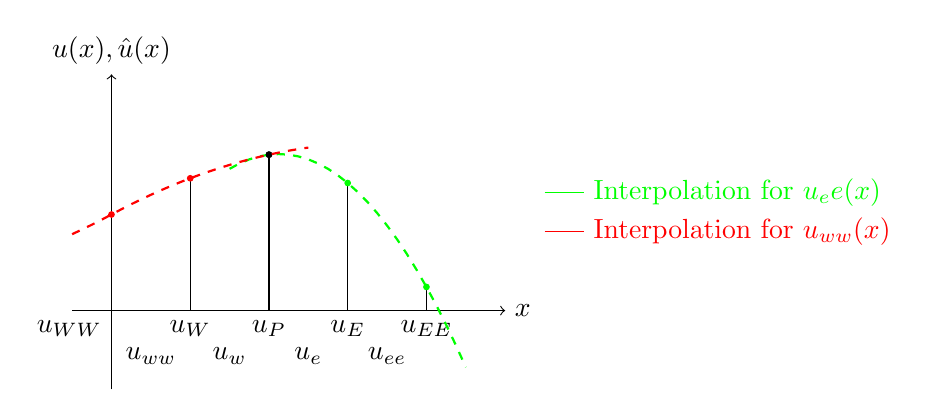
\begin{tikzpicture}

        \draw[->] (-0.5,0) -- (5,0) node[right] {$x$};
        \draw[->] (0,-1) -- (0,3) node[above] {$u(x), \hat{u}(x)$};

        % \draw [blue, thick] plot [smooth] coordinates {(-0.5,1) (2.5,2) (4.5,-0.5)};

        \draw (0,0) node[below left] {$u_{WW}$} -- (0,1.22);
        \draw (0.5,0) node[below, shift={(0,-10pt)}] {$u_{ww}$} -- (0.5,0);
        \draw (1,0) node[below] {$u_W$} -- (1,1.68);
        \draw (1.5,0) node[below, shift={(0,-10pt)}] {$u_w$} -- (1.5,0);
        \draw (2,0) node[below] {$u_P$} -- (2,1.98);
        \draw (2.5,0) node[below, shift={(0,-10pt)}] {$u_e$} -- (2.5,0);
        \draw (3,0) node[below] {$u_E$} -- (3,1.62);
        \draw (3.5,0) node[below, shift={(0,-10pt)}] {$u_{ee}$} -- (3.5,0);
        \draw (4,0) node[below] {$u_{EE}$} -- (4,0.3);

        % u_ee interpolation
        \filldraw[black] (2,1.98) circle (1pt);
        \filldraw[green] (3,1.62) circle (1pt);
        \filldraw[green] (4,0.3) circle (1pt);
        \draw [green, thick, dashed] plot[domain=1.5:4.5] (\x, {-0.48*\x^2 + 2.04*\x - 0.18});

        % w_ww interpolation
        \filldraw[red] (0,1.22) circle (1pt);
        \filldraw[red] (1,1.68) circle (1pt);
        \filldraw[black] (2,1.98) circle (1pt);
        \draw [red, thick, dashed] plot[domain=-0.5:2.5] (\x, {-0.08*\x^2 + 0.54*\x + 1.22});

        % Legend
        % \draw [blue] (5.5,2) -- (6,2) node[right] {Actual $\hat{u}(x)$};
        \draw [green] (5.5,1.5) -- (6,1.5) node[right] {Interpolation for $u_ee(x)$};
        \draw [red] (5.5,1) -- (6,1) node[right] {Interpolation for $u_{ww}(x)$};

    \end{tikzpicture}
    \caption{Example of the \acrshort{quick} scheme applied to the $u$ velocity component.}
    \label{fig:quick_convection_scheme}
\end{figure}

We can obtain a formula for the \acrshort{quick} that will be used in the implementation of the code.
In particular, we can recall the definition of the Lagrange interpolation polynomial of degree 2:

\begin{equation}
    P(x) = \sum_{i=0}^{2} y_i \prod_{j=0, j \neq i}^{2} \frac{x - x_j}{x_i - x_j}
    \label{eq:langrange_interpolation_polynomial}
\end{equation}

In our case, it's convenient to fix the reference system in correspondence of the center of the control volume considered.
If that is the case, then for example the evaluation of the velocity at the face $u_e$ will be:

\begin{equation}
    u_e = P(x) \bigg|_{x = \Delta x/2}
\end{equation}

As we said before, the choice of the interpolation points is based on the direction of the velocity at the face of the control volume.
In particular, if we are computing the $u_e$ velocity, the possible polynomials ($P_e(x)$) will be:

\begin{equation}
    P_e(x) = \begin{cases}
        P(u_W, u_P, u_E)    & \text{if } \hat{u_e} > 0 \\
        P(u_P, u_E, u_{EE}) & \text{if } \hat{u_e} < 0
    \end{cases}
\end{equation}

By using \texttt{Mathematica}, we can compute the polynomials for the $u$ velocity component in both cases.

The results of the symbolic analysis are:

\begin{align}
    u_e & = \begin{cases}
                -\frac{1}{8} u_W + \frac{3}{4} u_P + \frac{3}{8} u_E    & \text{if } \hat{u_e} > 0 \\
                +\frac{3}{8} u_P + \frac{3}{4} u_E - \frac{1}{8} u_{EE} & \text{if } \hat{u_e} < 0
            \end{cases}    \\
    u_w & = \begin{cases}
                -\frac{1}{8} u_{WW} +    \frac{3}{4} u_W + \frac{3}{8} u_P & \text{if } \hat{u_w} > 0 \\
                +\frac{3}{8} u_W + \frac{3}{4} u_P - \frac{1}{8} u_E       & \text{if } \hat{u_w} < 0
            \end{cases}
\end{align}

The same apply for the $v$ velocity component, but in this case, the variables that decide the interpolation points are the $\hat{v_n}$ and $\hat{v_s}$.

In the end, our \acrshort{quick} scheme applied to the convection term will be:

\begin{gather}
    \left(\hat{u_e}u_e - \hat{u_w}u_w\right) \Delta y + \left(\hat{v_n}u_n - \hat{v_s}u_s\right) \Delta x = \\
    \left(F_e u_e - F_w u_w\right) + \left(F_n u_n - F_s u_s\right) = \\
    \frac{1}{8} (
    (3 u_{E} + 6 u_{P} - u_{W}) max(0, F_e) + (- u_{EE} + 6 u_{E} + 3 u_{P}) min(0, F_e) + \\
    (- 3 u_{P} - 6 u_{W} + u_{WW}) max(0, F_w) + (u_{E} - 6 u_{P} - 3 u_{W}) min(0, F_w) + \\
    (3 u_{N} + 6 u_{P} - u_{S}) max(0, F_n) + (6 u_{N} - u_{NN} + 3 u_{P}) min(0, F_n) + \\
    (- 3 u_{P} - 6 u_{S} + u_{SS}) max(0, F_s) + (u_{N} - 6 u_{P} - 3 u_{S}) min(0, F_s)
    )
\end{gather}

Since we are interested in the $A_P^\phi$ and $A_{nb}^\phi$ coefficients as written in the form of Equation \ref{eq:coefficients_form_system}, with the help of \texttt{Mathematica}, we can regroup the terms based on the velocity components, perform some sign manipulations and obtain the coefficients for the convection term using the \acrshort{quick} scheme for both the $u$ and $v$ momentum equations.

\begin{equation*}
    \text{Convection Coefficients \acrshort{quick}:} = { \textbf{See table \ref{tab:Ap_coefficients}} }
\end{equation*}



%
% Hybrid scheme
%
\subsubsection{\acrfull{hybrid}}

The \acrfull{hybrid} combines the \acrshort{uds} and \acrshort{quick} schemes based on the Peclet number $P_e$.


\subsection{Diffusion Schemes}
\label{subsec:diffusion_schemes}

In this section, we will present the schemes related to the diffusion terms of the discretized governing equations, which were derived in Section \ref{subsec:application_of_the_finite_volume_method}.

The general idea here is to approximate the diffusion term using its Taylor expansion and then evaluate the derivative at the cell faces.
As a recall, the definition of the Taylor expansion of order $n$ is:

\begin{equation}
    f(x) = f(x_0) + f'(x_0)(x - x_0) + \frac{f''(x_0)}{2!}(x - x_0)^2 + \dots + \frac{f^n(x_0)}{n!}(x - x_0)^n + \mathbf{O}((x - x_0)^{n+1})
\end{equation}



%
% 2°-order scheme
%
\subsubsection{$2^{nd}$-order scheme}

The $2^{nd}$-order scheme approximate the diffusion term using the Taylor expansion up to the second order.

We can start by writing the polynomial that approximates by interpolation the values of the variable $u$ at the cell faces.
To do so, we can use the Lagrange interpolation polynomial, previously defined in Equation \ref{eq:langrange_interpolation_polynomial}.
Since we are now analyzing the $2^{nd}$-order scheme, we will use $n = 2+1 = 3$ points to interpolate.

As before, we can use \texttt{Mathematica} to obtain the polynomial that approximates function $u(x)$ as:

\begin{equation}
    u(x) \approx \frac{2 (\Delta x)^2 u_{P}+x^2 (u_{E}-2 u_{P}+u_{W})+\Delta x x (u_{E}-u_{W})}{2 (\Delta x)^2}
\end{equation}

We can now proceed by evaluating the second derivative of the polynomial as:

\begin{equation}
    \frac{\partial^2 u}{\partial x^2} \approx \frac{u_{E} - 2 u_{P} + u_{W}}{(\Delta x)^2}
\end{equation}

And finally, we can the approximated second derivative at the point of interest $x = 0$ as:

\begin{equation}
    \left. \frac{\partial^2 u}{\partial x^2} \right|_P \approx \frac{u_{E} - 2 u_{P} + u_{W}}{(\Delta x)^2}
\end{equation}

Given the definition of the diffusion term of $u$ along $x$ in Equation \ref{eq:INS_steady_2D_discretized_diffusion}, we can write the $2^{nd}$-order scheme as:

\begin{equation}
    \nu \frac{\partial^2 u}{\partial x^2} = \nu \frac{u_{E} - 2 u_{P} + u_{W}}{(\Delta x)^2}
\end{equation}

With a similar approach, we can obtain the $2^{nd}$-order scheme for the $y$ direction as:

\begin{equation}
    \nu \frac{\partial^2 u}{\partial y^2} = \nu \frac{u_{N} - 2 u_{P} + u_{S}}{(\Delta y)^2}
\end{equation}

The same procedure can be applied to the $v$ momentum equation, obtaining the following results:

\begin{gather}
    \nu \frac{\partial^2 u}{\partial x^2} + \nu \frac{\partial^2 u}{\partial y^2} = \\
    \frac{\Delta y \nu  (u_{E}-2 u_{P}+u_{W})}{\Delta x} + \\
    \frac{\Delta x \nu  (u_{N}-2 u_{P}+u_{S})}{\Delta y}
\end{gather}

Since we are interested in the $A_P^\phi$ and $A_{nb}^\phi$ coefficients as written in the form of Equation \ref{eq:coefficients_form_system}, with the help of \texttt{Mathematica}, we can regroup the terms based on the velocity components, perform some sign manipulations and obtain the coefficients for the diffusion term using the $2^{nd}$-order scheme for both the $u$ and $v$ momentum equations.

\begin{equation}
    \text{Diffusion Coefficients order} 2^{nd} = { \textbf{See table \ref{tab:Ap_coefficients}} }
\end{equation}



%
% 4°-order scheme
%
\subsubsection{$4^{th}$-order scheme}

The $4^{th}$-order scheme approximate the diffusion term using the Taylor expansion up to the fourth order.

Since the reasoning is similar to the $2^{nd}$-order scheme, we can directly write the approximated second derivative at the point of interest $x = 0$ as:

\begin{equation}
    \left. \frac{\partial^2 u}{\partial x^2} \right|_P \approx -\frac{u_{WW} - 16 u_{W} + 30 u_{P} - 16 u_{E} + u_{EE}}{12 (\Delta x)^2}
\end{equation}

Given the definition of the diffusion term of $u$ along $x$ in Equation \ref{eq:INS_steady_2D_discretized_diffusion}, we can write the $4^{th}$-order scheme as:

\begin{equation}
    \nu \frac{\partial^2 u}{\partial x^2} = \nu -\frac{u_{WW} - 16 u_{W} + 30 u_{P} - 16 u_{E} + u_{EE}}{12 (\Delta x)^2}
\end{equation}

With a similar approach, we can obtain the $4^{th}$-order scheme for the $y$ direction as:

\begin{equation}
    \nu \frac{\partial^2 u}{\partial y^2} = \nu -\frac{u_{WW} - 16 u_{W} + 30 u_{P} - 16 u_{E} + u_{EE}}{12 (\Delta y)^2}
\end{equation}

The same procedure can be applied to the $v$ momentum equation, obtaining the following results:

\begin{gather}
    \int_{V} \nu \frac{\partial^2 u}{\partial x^2} + \nu \frac{\partial^2 u}{\partial y^2} \space dV = \\
    -\frac{\nu}{12}  \left(\frac{u_{WW} - 16 u_{W} + 30 u_{P} - 16 u_{E} + u_{EE}}{(\Delta x)^2} + \frac{u_{WW} - 16 u_{W} + 30 u_{P} - 16 u_{E} + u_{EE}}{(\Delta y)^2} \right) \Delta x \Delta y
\end{gather}

Since we are interested in the $A_P^\phi$ and $A_{nb}^\phi$ coefficients as written in the form of Equation \ref{eq:coefficients_form_system}, with the help of \texttt{Mathematica}, we can regroup the terms based on the velocity components, perform some sign manipulations and obtain the coefficients for the diffusion term using the $4^{th}$-order scheme for both the $u$ and $v$ momentum equations.

\begin{equation}
    \text{Diffusion Coefficients order } 4^{th} = { \textbf{See table \ref{tab:Ap_coefficients}} }
\end{equation}

\subsection{Final coefficients}
\label{subsec:final_coefficients}

The final coefficients are obtained by reassembling the convection and diffusion coefficients, based on the FVM result:

\begin{equation}
    FVM_{\text{Convection}} - FVM_{\text{Diffusion}} = 0 \rightarrow (A^\phi) = (A^\phi)_{\text{Convection}} - (A^\phi)_{\text{Diffusion}}
\end{equation}


\eject
\newgeometry{margin=12mm}
\pdfpagewidth=275mm \pdfpageheight=150mm

\begin{center}
    \begin{table}[H]
        \centering
        \caption{Final $Ap$ coefficients for convection and diffusion using different schemes}
        \begin{tabular}{|l|l|l|l|l|l|}
            \hline
            \textbf{Ap}   & \textbf{Convection UDS} & \textbf{Convection CDS} & \textbf{Convection QUICK}                                                                     & \textbf{Diffusion 2° order}      & \textbf{Diffusion 4° order}          \\
            \hline
            $Ap\phi WWSS$ & $0$                     & $0$                     & $0$                                                                                           & $0$                              & $0$                                  \\
            $Ap\phi WWS$  & $0$                     & $0$                     & $0$                                                                                           & $0$                              & $0$                                  \\
            $Ap\phi WWP$  & $0$                     & $0$                     & $-\frac{1}{8} \max (0,Fw\phi )$                                                               & $0$                              & $-\frac{\Delta y \nu }{12 \Delta x}$ \\
            $Ap\phi WWN$  & $0$                     & $0$                     & $0$                                                                                           & $0$                              & $0$                                  \\
            $Ap\phi WWNN$ & $0$                     & $0$                     & $0$                                                                                           & $0$                              & $0$                                  \\
            $Ap\phi WSS$  & $0$                     & $0$                     & $0$                                                                                           & $0$                              & $0$                                  \\
            $Ap\phi WS$   & $0$                     & $0$                     & $0$                                                                                           & $0$                              & $0$                                  \\
            $Ap\phi WP$   & $\max (0,Fw\phi )$      & $\frac{Fw\phi}{2}$      & $\frac{1}{8} \max (0,Fe\phi )+\frac{3}{4} \max (0,Fw\phi )+\frac{3}{8} \min (0,Fw\phi )$      & $\frac{\Delta y \nu }{\Delta x}$ & $\frac{4 \Delta y \nu }{3 \Delta x}$ \\
            $Ap\phi WN$   & $0$                     & $0$                     & $0$                                                                                           & $0$                              & $0$                                  \\
            $Ap\phi WNN$  & $0$                     & $0$                     & $0$                                                                                           & $0$                              & $0$                                  \\
            $Ap\phi PSS$  & $0$                     & $0$                     & $-\frac{1}{8} \max (0,Fs\phi )$                                                               & $0$                              & $-\frac{\Delta x \nu }{12 \Delta y}$ \\
            $Ap\phi PS$   & $\max (0,Fs\phi )$      & $\frac{Fs\phi}{2}$      & $\frac{1}{8} \max (0,Fn\phi )+\frac{3}{4} \max (0,Fs\phi )+\frac{3}{8} \min (0,Fs\phi )$      & $\frac{\Delta x \nu }{\Delta y}$ & $\frac{4 \Delta x \nu }{3 \Delta y}$ \\
            \hline
            % $Ap\phi PP$   & $\max (0,Fe\phi )+\max (0,Fn\phi )-\min (0,Fs\phi )-\min (0,Fw\phi )$ & $\frac{Fe\phi}{2}+\frac{Fn\phi}{2}-\frac{Fs\phi}{2}-\frac{Fw\phi}{2}$ & $\frac{3}{4} \max (0,Fe\phi )+\frac{3}{8} \min (0,Fe\phi )+\frac{3}{4} \max (0,Fn\phi )+\frac{3}{8} \min (0,Fn\phi )-\frac{3}{8} \max (0,Fs\phi )-\frac{3}{4} \min (0,Fs\phi )-\frac{3}{8} \max (0,Fw\phi )-\frac{3}{4} \min (0,Fw\phi )$ & $-\Delta x \Delta y \nu  \left(-\frac{2}{\Delta x^2}-\frac{2}{\Delta y^2}\right)$ & $-\Delta x \Delta y \nu  \left(-\frac{5}{2 \Delta x^2}-\frac{5}{2 \Delta y^2}\right)$ \\
            $Ap\phi PP$   & $\sum_{nb} Ap\phi$      & $\sum_{nb} Ap\phi$      & $\sum_{nb} Ap\phi$                                                                            & $\sum_{nb} Ap\phi$               & $\sum_{nb} Ap\phi$                   \\
            \hline
            $Ap\phi PN$   & $-\min (0,Fn\phi )$     & $-\frac{Fn\phi}{2}$     & $\frac{1}{8} (-3) \max (0,Fn\phi )-\frac{3}{4} \min (0,Fn\phi )-\frac{1}{8} \min (0,Fs\phi )$ & $\frac{\Delta x \nu }{\Delta y}$ & $\frac{4 \Delta x \nu }{3 \Delta y}$ \\
            $Ap\phi PNN$  & $0$                     & $0$                     & $\frac{1}{8} \min (0,Fn\phi )$                                                                & $0$                              & $-\frac{\Delta x \nu }{12 \Delta y}$ \\
            $Ap\phi ESS$  & $0$                     & $0$                     & $0$                                                                                           & $0$                              & $0$                                  \\
            $Ap\phi ES$   & $0$                     & $0$                     & $0$                                                                                           & $0$                              & $0$                                  \\
            $Ap\phi EP$   & $-\min (0,Fe\phi )$     & $-\frac{Fe\phi}{2}$     & $\frac{1}{8} (-3) \max (0,Fe\phi )-\frac{3}{4} \min (0,Fe\phi )-\frac{1}{8} \min (0,Fw\phi )$ & $\frac{\Delta y \nu }{\Delta x}$ & $\frac{4 \Delta y \nu }{3 \Delta x}$ \\
            $Ap\phi EN$   & $0$                     & $0$                     & $0$                                                                                           & $0$                              & $0$                                  \\
            $Ap\phi ENN$  & $0$                     & $0$                     & $0$                                                                                           & $0$                              & $0$                                  \\
            $Ap\phi EESS$ & $0$                     & $0$                     & $0$                                                                                           & $0$                              & $0$                                  \\
            $Ap\phi EES$  & $0$                     & $0$                     & $0$                                                                                           & $0$                              & $0$                                  \\
            $Ap\phi EEP$  & $0$                     & $0$                     & $\frac{1}{8} \min (0,Fe\phi )$                                                                & $0$                              & $-\frac{\Delta y \nu }{12 \Delta x}$ \\
            $Ap\phi EEN$  & $0$                     & $0$                     & $0$                                                                                           & $0$                              & $0$                                  \\
            $Ap\phi EENN$ & $0$                     & $0$                     & $0$                                                                                           & $0$                              & $0$                                  \\
            \hline
        \end{tabular}
        \label{tab:Ap_coefficients}
    \end{table}
\end{center}

\eject
\restoregeometry
\pdfpagewidth=210mm
\pdfpageheight=297mm

\section{\acrfull{scgs}}
\label{sec:scgs}

So far we have presented the set of differential equations that govern the fluid flow, and we have also discretized them using the FVM and applying different schemes (for the convection and diffusion terms).

In the following we will discuss the \acrfull{scgs} method by \cite[Vanka (1986)]{VANKA1986138}, which combine all the information we have presented so far, and will allow us to solve the discretized equations iteratively.

Notice that when we say \textit{solve the equations}, we mean to find the values of the velocity components and the pressure at each cell of the domain, namely $U(x_i, y_j)$ \& $V(x_i, y_j)$ \& $P(x_i, y_j)$, so to have a complete description of the flow field.

\subsection{Variable Correction Concept}
\label{subsec:variable_correction_concept}

Before presenting the \acrshort{scgs} method itself, it's now useful to introduce the concept of variable correction, which is crucial for the understanding of the method.

The idea here is to observe a generic current state of the system $\phi^{(n)}$, as the sum of a known part $\phi^{(n-1)}$ and a correction $\delta \phi^{(n)}$:

\begin{equation}
    \phi^{(n)} = \phi^{(n-1)} + \delta \phi^{(n)}
    \label{eq:variable_correction_concept}
\end{equation}

Where $\phi$ is a generic variable, and $n$ is the iteration index.

For simplicity of notation, we will drop the iteration index in the following, and we will rewrite Equation \ref{eq:variable_correction_concept} as:

\begin{equation}
    \phi = \phi^* + \phi'
    \label{eq:variable_correction_concept_simplified}
\end{equation}

Where $\phi^*$ is the known part, and $\phi'$ is the correction.

By doing so, we can rewrite the state of the system at the current iteration as:

\begin{align}
    u_{i,j} & = u_{i,j}^* + u_{i,j}' \\
    v_{i,j} & = v_{i,j}^* + v_{i,j}' \\
    p_{i,j} & = p_{i,j}^* + p_{i,j}'
    \label{eq:variable_corrections}
\end{align}
\subsection{Equations Coupling}
\label{subsec:equations_coupling}

At this point, one could ask how the three equations we have presented so far are related to each other.
The answer is in the continuity equation, which is the key to couple the velocity and pressure fields (and indeed, have a close form of the system with 3 equations \ref{eq:INS_steady_2D_discretized_continuity_final} \ref{eq:INS_steady_2D_discretized_momentum_x_final} \ref{eq:INS_steady_2D_discretized_momentum_y_final} and 3 unknowns).

Given that the continuity equation is defined for a given $p-CV$ and that involve the all the four velocity components at the faces of the control volume, it should be intuitive that in order to solve the equilibrium across one cell, we need to have a system of equations that involve all the four velocity components.

By recalling the representation with index notation for the $p-CV$, we can compose our system of equations.

\begin{figure}[H]
    \centering
    \def\nCV{1}
    \def\dX{5cm}
    \def\dY{5cm}

    \begin{tikzpicture}[every node/.style={font=\huge}]

        \draw (0, 0) -- ++(\dX, 0) -- ++(0, \dY) -- ++(-\dX, 0) -- cycle;

        \node at (\dX/2, \dY/2) {$P_{i,j}$};
        \draw[thick, red, ->] (\dX/2, \dY/2)++(\dX/4, 0) -- ++(\dX/2, 0) node[pos=1, above] {$u_{i,j}$};
        \draw[thick, red, ->] (\dX/2, \dY/2)++(-\dX/2-\dX/4, 0) -- ++(\dX/2, 0) node[pos=0, above] {$u_{i-1,j}$};
        \draw[thick, blue, ->] (\dX/2, \dY/2)++(0,  \dY/4) -- ++(0, \dY/2) node[pos=1, right] {$v_{i,j}$};
        \draw[thick, blue, ->] (\dX/2, \dY/2)++(0, -\dY/2-\dY/4) -- ++(0, \dY/2) node[pos=0, right] {$v_{i,j-1}$};

        \node at (\dX/7, \dY/10) {$i,j$};

    \end{tikzpicture}
    \caption{Generic $p-CV$ with the velocity components at the faces.}
\end{figure}

\begin{equation}
    \begin{cases}
        \text{Mom. } u_{i-1, j} \\
        \text{Mom. } u_{i, j}   \\
        \text{Mom. } v_{i, j-1} \\
        \text{Mom. } v_{i, j}   \\
        \text{Con.}
    \end{cases}
    =
    \begin{cases}
        (A_P^u)_{i-1,j} u_{i-1,j}                                       & = \sum_{nb} (A_{nb}^u)_{i-1,j} (u_{nb})_{i-1,j} + (p_{i-1,j} - p_{i,j}) \Delta y \\
        (A_P^u)_{i,j} u_{i,j}                                           & = \sum_{nb} (A_{nb}^u)_{i,j} (u_{nb})_{i,j} + (p_{i,j} - p_{i+1,j}) \Delta y     \\
        (A_P^v)_{i,j-1} v_{i,j-1}                                       & = \sum_{nb} (A_{nb}^v)_{i,j-1} (v_{nb})_{i,j-1} + (p_{i,j-1} - p_{i,j}) \Delta x \\
        (A_P^v)_{i,j} v_{i,j}                                           & = \sum_{nb} (A_{nb}^v)_{i,j} (v_{nb})_{i,j} + (p_{i,j} - p_{i,j+1}) \Delta x     \\
        (u_{i,j} - u_{i-1,j}) \Delta y + (v_{i,j} - v_{i,j-1}) \Delta x & = 0
    \end{cases}
\end{equation}

The system of equations is composed by 5 equations and 5 unknowns ($u_{i-1,j}$, $u_{i,j}$, $v_{i,j-1}$, $v_{i,j}$, $p_{i,j}$), and it's the result of the coupling of the momentum and continuity equations across a generic $p-CV$.
\subsection{Residual Concept}
\label{subsec:residual_concept}

Being the \acrshort{scgs} an iterative method, it's crucial to introduce the concept of residual, which is the key to understand the convergence of the method.

The residual is the difference between the left-hand side and the right-hand side of the discretized equations, and it's a measure of the error of the current state of the system.

For our system of 5 equations, we can define 5 residuals, one for each equation.

To simplify the set of equations (and have a simpler matrix resolution afterwards), we can choose to apply the correction to only some variables, and not to all of them.

In particular, we can choose to neglect the correction for the velocity and pressure components regarding the neighbor cells, and apply the correction only to the pressure and the velocity components at the current cell.

By doing so, we can rewrite the system of equations as:

\begin{gather}
    (A_P^u)_{i-1,j} (u_{i-1,j}^*+u_{i-1,j}') = \sum_{nb} (A_{nb}^u)_{i-1,j} (u_{nb}^*)_{i-1,j} + (p_{i-1,j}^* - (p_{i,j}^* + p_{i,j}')) \Delta y \\
    (A_P^u)_{i,j}   (u_{i,j}  ^*+u_{i,j}')   = \sum_{nb} (A_{nb}^u)_{i,j} (u_{nb}^*)_{i,j}     + ((p_{i,j}^* + p_{i,j}') - p_{i+1,j}^*) \Delta y   \\
    (A_P^v)_{i,j-1} (v_{i,j-1}^*+v_{i,j-1}') = \sum_{nb} (A_{nb}^v)_{i,j-1} (v_{nb}^*)_{i,j-1} + (p_{i,j-1}^* - (p_{i,j}^* + p_{i,j}')) \Delta x \\
    (A_P^v)_{i,j}   (v_{i,j}  ^*+v_{i,j}')   = \sum_{nb} (A_{nb}^v)_{i,j} (v_{nb}^*)_{i,j}     + ((p_{i,j}^* + p_{i,j}') - p_{i,j+1}^*) \Delta x   \\
    ((u_{i,j}  ^*+u_{i,j}') - (u_{i-1,j}^*+u_{i-1,j}')) \Delta y + ((v_{i,j}  ^*+v_{i,j}') - (v_{i,j-1}^*+v_{i,j-1}')) \Delta x = 0
\end{gather}

As explained in Subsection \ref{subsec:variable_correction_concept}, the $^*$ superscript is used to indicate the value of the variable at the previous iteration, and the $'$ superscript is used to indicate the correction to apply to the variable.
This means that the $\phi^*$ are known values, and the $\phi'$ are the unknowns to solve for.

We can now rearrange each equation to have the unknowns on the left-hand side and the known on the right-hand side:

\begin{align}
    (A_P^u)_{i-1,j} u_{i-1,j}' + p_{i,j}' \Delta y                      & = R^u_{i-1,j} \\
    (A_P^u)_{i,j}   u_{i,j}'   - p_{i,j}'   \Delta y                    & = R^u_{i,j}   \\
    (A_P^v)_{i,j-1} v_{i,j-1}' + p_{i,j}' \Delta x                      & = R^v_{i,j-1} \\
    (A_P^v)_{i,j}   v_{i,j}'   - p_{i,j}'   \Delta x                    & = R^v_{i,j}   \\
    (u_{i,j}' - u_{i-1,j}') \Delta y + (v_{i,j}' - v_{i,j-1}') \Delta x & = R^c_{i,j}
    \label{eq:residual_system}
\end{align}

Where $R^\phi_{i,j}$ is the residual of the $\phi$ equation at the $i,j$ cell.

The residuals, computed from the previous system by moving the known terms to the right-hand side, are defined as:

\begin{align}
    R^u_{i-1,j} & = \sum_{nb} (A_{nb}^u)_{i-1,j} (u_{nb}^*)_{i-1,j} - (A_P^u)_{i-1,j} u_{i-1,j}^*   + (p_{i-1,j}^* - p_{i,j}^*) \Delta y \\
    R^u_{i,j}   & = \sum_{nb} (A_{nb}^u)_{i,j} (u_{nb}^*)_{i,j} - (A_P^u)_{i,j} u_{i,j}^*           + (p_{i,j}^* - p_{i+1,j}^*) \Delta y \\
    R^v_{i,j-1} & = \sum_{nb} (A_{nb}^v)_{i,j-1} (v_{nb}^*)_{i,j-1} - (A_P^v)_{i,j-1} v_{i,j-1}^*   + (p_{i,j-1}^* - p_{i,j}^*) \Delta x \\
    R^v_{i,j}   & = \sum_{nb} (A_{nb}^v)_{i,j} (v_{nb}^*)_{i,j} - (A_P^v)_{i,j} v_{i,j}^*           + (p_{i,j}^* - p_{i,j+1}^*) \Delta x \\
    R^c_{i,j}   & = -\left[(u_{i,j}^* - u_{i-1,j}^*) \Delta y + (v_{i,j}^* - v_{i,j-1}^*) \Delta x\right]
\end{align}


\subsection{Gauss-Seidel Iterative Method}
\label{subsec:gauss_seidel_iterative_method}

Before, proceeding with the solution of the \acrshort{scgs} method, we need to introduce the \acrfull{gs} method.

The \acrshort{gs} method is an iterative method used to solve a system of linear equations, and it's based on the idea of solving one equation at a time, and using the updated values of the variables to solve the next equation.

For our purpose, is interesting to observe how the introduction of the 'under-relaxation' factor $\alpha$ can help to improve the convergence of the method.

In particular, we can apply the \acrshort{gs} method to solve a similar equation of our system, as for example:

\begin{equation}
    (A_P^\phi) \phi_P = \sum_{nb} (A_{nb}^\phi) \phi_{nb} + S^\phi
\end{equation}

Where $\phi$ is a generic variable, and $S^\phi$ is the source term of the equation.

The \acrshort{gs} method can be written as:

\begin{align}
    \phi_P & = \frac{\sum_{nb} (A_{nb}^\phi) \phi_{nb}^* + S^\phi}{A_P^\phi} + \phi_P^*                                \\
    \phi_P & = \alpha \left(\frac{\sum_{nb} (A_{nb}^\phi) \phi_{nb}^* + S^\phi}{A_P^\phi} - \phi_P^*\right) + \phi_P^*
\end{align}

Where $\phi_P^*$ is the value of the variable at the previous iteration, and $\alpha$ is the under-relaxation factor.

By rearranging the last equation, we have:

\begin{equation}
    \phi_P' = \frac{R_P^\phi}{\left(\frac{A_P^\phi}{\alpha_\phi}\right)}
\end{equation}

Where $\phi_P'$ is the correction to apply to the variable, and $R_P^\phi$ is the residual of the equation at the $P$ cell.

This result will be useful in the next section.

\subsection{Vanka's approach}
\label{subsec:vanka_approach}

The \acrshort{scgs} method is based on the idea of solving the equations in a coupled way.

This means that for each iteration, we will obtain the correction for each of the 5 variables simultaneously.
To make this possible, we need to introduce a new matrix, called the \textbf{Vanka matrix \cite{VANKA1986138}}.

Considering the system of equations \ref{eq:residual_system}, we can write them in a matrix form as:

\begin{equation}
    \begin{bmatrix}
        (A_P^u)_{i-1,j} & 0             & 0               & 0             & \Delta y  \\
        0               & (A_P^u)_{i,j} & 0               & 0             & -\Delta y \\
        0               & 0             & (A_P^v)_{i,j-1} & 0             & \Delta x  \\
        0               & 0             & 0               & (A_P^v)_{i,j} & -\Delta x \\
        -\Delta y       & \Delta y      & -\Delta x       & \Delta x      & 0
    \end{bmatrix}
    \begin{bmatrix}
        u'_{i-1,j} \\
        u'_{i,j}   \\
        v'_{i,j-1} \\
        v'_{i,j}   \\
        p'_{i,j}
    \end{bmatrix}
    =
    \begin{bmatrix}
        R_{i-1,j}^u \\
        R_{i,j}^u   \\
        R_{i,j-1}^v \\
        R_{i,j}^v   \\
        R_{i,j}^c
    \end{bmatrix}
    \label{eq:vanka_matrix}
\end{equation}

As we can see, the Vanka matrix is a $5 \times 5$ matrix, and it's a function of the coefficients of the discretized equations, and of the grid spacing.

Our unknown is the vector of the corrections, being the $A_P^\phi$ coefficients and the $R^\phi$ residuals known from the previous iteration.

Given that, we can solve the system of equations \ref{eq:vanka_matrix} to obtain the corrections for the velocity and pressure components at each cell of the domain.

To do so, we must invert the Vanka matrix, and multiply it by the residuals vector:

\begin{equation}
    \begin{bmatrix}
        \phi'
    \end{bmatrix}
    =
    \begin{bmatrix}
        A^\phi
    \end{bmatrix}^{-1}
    \begin{bmatrix}
        R^\phi
    \end{bmatrix}
\end{equation}

As stated in \cite{VANKA1986138}, the inverse of the Vanka matrix can be computed analytically using the following algorithm:

\begin{gather}
    r_i = \frac{a_{5i}}{a_{ii}}, \quad i = 1, 2, 3, 4 \\
    DEN = \sum_{i=1}^{4} a_{5i} r_i \\
    x_5 = \frac{\left[\sum_{i=1}^{4} r_i b_i - b_5\right]}{DEN} \\
    x_i = \frac{b_i - a_{i5} x_5}{a_{ii}}, \quad i = 1, 2, 3, 4
\end{gather}

Where $a_{ij}$ are the elements of the Vanka matrix $A^\phi$, $b_i$ are the elements of the residuals vector $R^\phi$, and $x_i$ are the elements of the corrections vector $\phi'$.

In case we want to apply an under-relaxation factor to the corrections, we can modify Vanka's Matrix as follows:

\begin{equation}
    \begin{bmatrix}
        \frac{(A_P^u)_{i-1,j}}{\alpha_u} & 0                              & 0                                & 0                              & \Delta y  \\
        0                                & \frac{(A_P^u)_{i,j}}{\alpha_u} & 0                                & 0                              & -\Delta y \\
        0                                & 0                              & \frac{(A_P^v)_{i,j-1}}{\alpha_v} & 0                              & \Delta x  \\
        0                                & 0                              & 0                                & \frac{(A_P^v)_{i,j}}{\alpha_v} & -\Delta x \\
        -\Delta y                        & \Delta y                       & -\Delta x                        & \Delta x                       & 0
    \end{bmatrix}
\end{equation}

Where $\alpha_u$ and $\alpha_v$ are the under-relaxation factors for the velocity components $u$ and $v$ respectively.
\subsection{Boundary conditions for Lid-Driven Cavity problem}
\label{subsec:boundary_conditions_for_lid_driven}

So far, we have presented all the tools and concepts required to solve a generic fluid flow problem (except for the algorithm itself) that respect the hypothesis and conditions stated at the beginning of Section \ref{sec:derivation_of_discretized_governing_equations}.

In this section we will present the boundary conditions that will be used to solve the Lid-Driven Cavity problem and their implementation inside the \acrshort{scgs} method.



\subsubsection{Ghosts cells}

Consider that our domain has already been discretized (subdivided) into $N_x \times N_y$ cells.

If we think of the scheme for both the convection and diffusion presented before, we can see that at the boundary of our domain, the coefficients $A_p\phi$ \ref{tab:Ap_coefficients} involve cells that are outside the domain.
For this reason, we need to add a layer of cells outside the physical domain, called ghost cells, to calculate the coefficients at the boundary.

The number of ghost cells required depends on the order of the scheme used to calculate the coefficients. For a second-order scheme, we need at least one ghost cell, and for a fourth-order scheme, we need at least two ghost cells.

Here, and also in the implementation of the \acrshort{scgs} method in the code, we will consider the possibility to adopt a mixed strategy scheme and use:

\begin{itemize}
    \item Away from boundaries: higher-order schemes
    \item Near boundaries: \acrshort{uds} scheme for convection and 2nd-order scheme for diffusion
\end{itemize}

By doing so, we ensure that at the boundaries both the schemes will be applicable with just a single layer of ghost cells.

\begin{figure}[H]
    \centering
    \def\nCV{5}
    \def\dX{1.5cm}
    \def\dY{1.5cm}

    \begin{tikzpicture}

        \foreach \n in {0,1,...,\nCV}
            {
                \draw (0, \n*\dY) -- (\nCV*\dX, \n*\dY);
                \draw (\n*\dX, 0) -- (\n*\dX, \nCV*\dY);
            }

        % \foreach \n in {0,1,...,\the\numexpr\nCV-1\relax}
        %     {
        %         \draw[dashed] (-\dX/2, \n*\dY + \dY/2) -- (\nCV*\dX+\dX/2, \n*\dY + \dY/2);
        %         \draw[dashed] (\n*\dX + \dX/2, -\dY/2) -- (\n*\dX + \dX/2, \nCV*\dY+\dY/2);
        %     }

        \foreach \y in {0,1,...,\the\numexpr\nCV-1\relax}
            {
                \foreach \x in {0,1,...,\the\numexpr\nCV-1\relax}
                    {
                        \node[font=\small] at (\x*\dX+\dX/6, \y*\dY+\dY/10) {$_{\the\numexpr\x+0\relax,\the\numexpr\y+0\relax}$};
                    }
            }

        \draw[line width=0.5mm] (\dX, \dY) -- (\dX, \nCV*\dY-\dY) -- (\nCV*\dX-\dX, \nCV*\dY-\dY) -- (\nCV*\dX-\dX, \dY) -- cycle;

        % \fill[red, opacity=0.1] (0, 0) rectangle (\nCV*\dX, \nCV*\dY);
        \fill[yellow, opacity=0.3] (\dX, \dY) rectangle (\nCV*\dX-\dX, \nCV*\dY-\dY);

    \end{tikzpicture}
    \caption{Physical domain and ghost cells}
    \label{fig:ghost_cells}
\end{figure}

In Figure \ref{fig:ghost_cells}, the yellow area represents the physical domain, while the frame surrounding it represents the ghost cells.

As we can see, the indexes of the cells stick to the physical domain, while the ghost cells may have negative indexes.

In the case above, we can declare some of the problem that will be recalled during the following sections:

\begin{itemize}
    \item Physical domain: $N_x \times N_y$ grid. In the example above, $N_x = N_y = 3$
    \item Physical domain indexes: from $(1,1)$ to $(3,3)$. In general, from $(1,1)$ to $(N_x,N_y)$.
    \item Ghost cells layer: may have different sizes along the $x$ and $y$ directions. In the example above, the ghost cells layer has a size of $N_g = 1$ cell in both directions. We will stick with this size for the rest of the document.
    \item Ghost cells indexes: may have negative indexes. In the example above, the ghost cells have indexes from $(0,0)$ to $(4,4)$, that is equivalent to $(1-N_g,1-N_g)$ to $(N_x+2*N_g-1,N_y+2*N_g-1)$.
\end{itemize}

We can now proceed to identify the boundary conditions for the Lid-Driven Cavity problem.



\subsubsection{No-slip condition}

As boundary conditions for the Lid-Driven Cavity problem (and for most of the fluid flow problems), we have the no-slip condition, which gives us the constraint for two direction of the velocity field:

\begin{itemize}
    \item Component normal to the wall: given a condition of impenetrability, the velocity component normal to the wall must be zero (no-penetration)
    \item Component tangential to the wall: given a condition of no-slip, the velocity component tangential to the wall must equal to the wall velocity
\end{itemize}

As an example, we can consider the cell in position $(1, N_y)$, which is the top-left corner of the physical domain (Figure \ref{fig:ghost_cells} for reference).

\begin{figure}[H]
    \centering
    \def\nCV{2}
    \def\dX{3cm}
    \def\dY{3cm}

    \begin{tikzpicture}

        \foreach \n in {0,1,...,\nCV}
            {
                \draw (0, \n*\dY) -- (\nCV*\dX, \n*\dY);
                \draw (\n*\dX, 0) -- (\n*\dX, \nCV*\dY);
            }

        \foreach \y in {0,1,...,\the\numexpr\nCV-1\relax}
            {
                \foreach \x in {0,1,...,\the\numexpr\nCV-1\relax}
                    {
                        \node[font=\small] at (\x*\dX+\dX/5, \y*\dY+\dY/15) {$_{\x, N_y+\y}$};
                    }
            }

        \draw[thick, blue, ->] (3/2*\dX, 1/2*\dY)++(0,  \dY/4) -- ++(0, \dY/2) node[pos=1, right] {$v_{1,N_y}$};
        \draw[thick, blue, ->] (3/2*\dX, 1/2*\dY)++(0, -\dY/2-\dY/4) -- ++(0, \dY/2) node[pos=1, right] {$v_{1,N_y-1}$};
        \draw[thick, red, ->] (3/2*\dX, 1/2*\dY)++(\dX/4, 0) -- ++(\dX/2, 0) node[pos=1, above] {$u_{1,N_y}$};
        \draw[thick, red, ->] (3/2*\dX, 1/2*\dY)++(-\dX/2-\dX/4, 0) -- ++(\dX/2, 0) node[pos=1, above] {$u_{0,N_y}$};

        \fill[yellow, opacity=0.3] (\dX, 0) rectangle (2*\dX, \dY);

        \draw[line width=1mm] (\dX, -\dY/10) -- (\dX, \dY) -- (2*\dX+\dX/10, \dY);
        \draw[thick, ->] (2*\dX +\dX/10, \dY) ++(\dX/5, 0) -- ++(\dX/2, 0) node[pos=1, above] {$U_{lid}$};

    \end{tikzpicture}
    \caption{Boundary conditions for the cell $(1, N_y)$}
    \label{fig:boundary_conditions_1Ny}
\end{figure}

In this case, we must accomplish the following conditions:

\begin{itemize}
    \item $u_{0, N_y} = 0$ (no-penetration)
    \item $v_{1, N_y} = 0$ (no-penetration)
    \item $u_{1, N_y} = U_{lid}$ (no-slip)
\end{itemize}

Intuitively, we can understand that similar conditions must be applied to the other walls of the domain given the correction of the indexes and the direction of the velocity field.

In general, we can state that the boundary conditions for the Lid-Driven Cavity problem are:

\begin{itemize}
    \item Bottom wall: $v_{i,0} = 0$ (no-penetration) + $u_{i,1} = 0$ (no-slip)
    \item Left wall: $u_{0,j} = 0$ (no-penetration) + $v_{1,j} = 0$ (no-slip)
    \item Top wall: $v_{i,N_y} = 0$ (no-penetration) + $u_{i,N_y} = U_{lid}$ (no-slip)
    \item Right wall: $u_{N_x,j} = 0$ (no-penetration) + $v_{N_x,j} = 0$ (no-slip)
\end{itemize}

We can now proceed to see how these conditions are accounted for in the \acrshort{scgs} method.



\subsubsection{Boundary conditions inside \acrshort{scgs} method}

By adopting the \acrshort{scgs} method, we can impose the boundary conditions in the following way:

\begin{itemize}
    \item No-penetration condition: impose specific coefficients in the Vanka matrix to be zero
    \item No-slip condition: impose specific velocity values in the ghost cells
\end{itemize}

Moreover, as we are going to see, the no-penetration condition imply the velocity to be null and can be imposed to the system before solving the linear system of equations.
Instead, given the mathematical formulation of the no-slip condition, we can impose the velocity values in the ghost cells only after solving the linear system of equations (and will affect the next iteration).

\paragraph{No-penetration condition}

The no-penetration condition imply the normal velocity component at the boundary to be null.
This means that if we start from an initial guess of the velocity field equal to zero everywhere, we must ensure that correction of the velocity field at the boundary is null for each iteration.

Taken for example the cell $(1, N_y)$ as in Figure \ref{fig:boundary_conditions_1Ny}, we know that we must impose $u_{0, N_y} = 0$ \& $v_{1, N_y} = 0$, which means that the correction of the velocity field at the boundary must be null as well $u_{0, N_y}' = 0$ \& $v_{1, N_y}' = 0$.

By recalling the formulation for both the continuity and momentum equations, we can see that multiple terms must be canceled out (known null solution).

For the \textbf{continuity equation} written at the cell $(1, N_y)$, we have:

\begin{equation}
    -u_{0, N_y}' \Delta y + u_{1, N_y}' \Delta y - v_{1, N_y-1}' \Delta x + v_{1, N_y}' \Delta x = R_{1, N_y}^c
\end{equation}

By imposing $[A^\phi]_{5,1} = \Delta y = 0$, we can cancel out the first term, and by imposing $[A^\phi]_{5, 4} = \Delta x = 0$, we can cancel out the third term.

In this way, even if we are not imposing the no-penetration condition directly, we are imposing an equivalent condition that will lead to the same result.

More in general, given the physical domain of size $N_x \times N_y$, we can impose the no-penetration condition for the continuity equation by setting:

\begin{align}
    @i=1, u_{i-1, j}' = 0 \rightarrow [A^\phi]_{5,1} & = - \Delta y = 0 \quad \forall j = 1,2,...,N_y \\
    @i=N_x, u_{i, j}' = 0 \rightarrow [A^\phi]_{5,2} & = \Delta y = 0 \quad \forall j = 1,2,...,N_y   \\
    @j=1, v_{i, j-1}' = 0 \rightarrow [A^\phi]_{5,3} & = - \Delta x = 0 \quad \forall i = 1,2,...,N_x \\
    @j=N_y, v_{i, j}' = 0 \rightarrow [A^\phi]_{5,4} & = \Delta x = 0 \quad \forall i = 1,2,...,N_x
\end{align}

For the \textbf{momentum equations}, written at the cell $(1, N_y)$ for the two components that are controlled by the no-penetration condition, we have:

\begin{align}
    (A_P^u)_{0,N_y} u_{0,N_y}' + p_{0,N_y}' \Delta y & = R^u_{0,N_y} \\
    (A_P^v)_{1,N_y} v_{1,N_y}' - p_{1,N_y}' \Delta x & = R^v_{1,N_y}
\end{align}

By imposing $[A^\phi]_{1,5} = \Delta y = 0$ and $[R^\phi]_{1} = 0$, we can cancel out the first equation, and by imposing $[A^\phi]_{4,5} = - \Delta x = 0$ and $[R^\phi]_{4} = 0$, we can cancel out the second equation.

More in general, given the physical domain of size $N_x \times N_y$, we can impose the no-penetration condition for the momentum equations by setting:

\begin{align}
    @i=1, u_{i-1, j}' = 0 \rightarrow [A^\phi]_{1,5} & = \Delta y = 0 \quad \forall j = 1,2,...,N_y   \\
    @i=N_x, u_{i, j}' = 0 \rightarrow [A^\phi]_{2,5} & = - \Delta y = 0 \quad \forall j = 1,2,...,N_y \\
    @j=1, v_{i, j-1}' = 0 \rightarrow [A^\phi]_{3,5} & = \Delta x = 0 \quad \forall i = 1,2,...,N_x   \\
    @j=N_y, v_{i, j}' = 0 \rightarrow [A^\phi]_{4,5} & = - \Delta x = 0 \quad \forall i = 1,2,...,N_x
\end{align}

\paragraph{No-slip condition}

The idea behind the no-slip condition for the tangential velocity component is to impose the velocity field in the ghost cells so that the interpolation with the velocity field in the physical domain gives the correct value at the boundary.

As an example, we can consider the cell $(1, N_y)$ as in Figure \ref{fig:boundary_conditions_1Ny}.

We know that we must impose $u_{1, N_y} = U_{lid}$.
Given that the condition can't be imposed directly to the correction term as for the no-penetration condition, here we have to solve the system and then impose the condition over the ghost cells velocity based on the current solution of the velocity field.

In particular, we can think of the wall velocity as the average of the velocity in the ghost cell and the velocity in the physical domain.
This implies to impose the following condition for the cell $(1, N_y)$:

\begin{equation}
    U_{lid} = \frac{1}{2} (u_{1, N_y} + u_{1, N_y+1}) \rightarrow u_{1, N_y+1} = 2 U_{lid} - u_{1, N_y}
\end{equation}

More in general, given the physical domain of size $N_x \times N_y$, we can impose the no-slip condition for the velocity field by setting:

\begin{align}
    @i=1, v_{0, j}       & = - v_{1, j} \quad \forall j = 1,2,...,N_y             \\
    @i=N_x, v_{N_x+1, j} & = - v_{N_x, j} \quad \forall j = 1,2,...,N_y           \\
    @j=1, u_{i, 0}       & = - u_{i, 1} \quad \forall i = 1,2,...,N_x             \\
    @j=N_y, u_{i, N_y+1} & = 2 U_{lid} - u_{i, N_y} \quad \forall i = 1,2,...,N_x
\end{align}
\subsection{Convergence criterion}
\label{sec:convergence_criterion}

Being the \acrshort{scgs} method an iterative method, we need to define a criterion to stop the iterations, and to consider the solution as converged.

We could have adopted many criteria, but probably the most intuitive one is to monitor the residuals of the equations over the entire domain for each iteration, and to stop the cycle when the maximum of the residual is below a certain threshold.

So far we have defined 5 residuals, one for each equation, and we can define other 3 residuals derived from the previous ones, as follows:

\begin{equation}
    \begin{aligned}
        \text{Continuity residual} & : R^p = | R^c |                                               \\
        \text{Momentum residual u} & : R^u = \frac{\left( | R_{i-1}^u | + | R_{i}^u | \right) }{2} \\
        \text{Momentum residual v} & : R^v = \frac{\left( | R_{j-1}^v | + | R_{j}^v | \right) }{2}
    \end{aligned}
\end{equation}

By doing so, our convergence criterion will be:

\begin{equation}
    \max \left( R^p, R^u, R^v \right) < \varepsilon
\end{equation}

Where $\varepsilon$ is the threshold and may vary between $10^{-3}$ and $10^{-6}$, depending on the problem and the computational resources available.


\section{Code implementation}
\label{sec:code_implementation}

When it comes to the implementation of the \acrshort{scgs} and \acrshort{simple} algorithms, lots of details need to be taken into account, such as the data structures, the memory allocation, the data exchange between the different modules of the code, and so on.

% In the following, we report the core of the \acrshort{scgs} algorithm, both in a flowchart and in a \texttt{C} implementation.
% In the following, we report the core of the \acrshort{scgs} algorithm in a \texttt{C} implementation.

The complete codebase is available on GitHub at \url{https://github.com/Bocchio01/CFD_Simulation_Engine}.

% \begin{figure}[H]
%     \centering

%     \tikzstyle{decision} = [diamond, draw, fill=red!20, text width=4.5em, text badly centered, node distance=3cm, inner sep=0pt]
%     \tikzstyle{block} = [rectangle, draw, fill=blue!20, text width=5em, text centered, rounded corners, minimum height=4em]
%     \tikzstyle{line} = [draw, -latex']

%     \begin{tikzpicture}[node distance = 2cm, auto]
%         % Place nodes
%         \node [block] (init) {Allocate Memory};
%         \node [block, below of=init] (reset) {Reset SCGS};
%         \node [block, below of=reset] (compose) {Compose System Matrix};
%         \node [block, below of=compose] (noslip) {Apply Normal No-Slip BCs};
%         \node [block, below of=noslip] (solve) {Solve System Matrix};
%         \node [block, below of=solve] (correct) {Apply Corrections};
%         \node [block, below of=correct] (residuals) {Update Residuals};
%         \node [block, below of=residuals] (noslipt) {Apply Tangential No-Slip BCs};
%         \node [decision, below of=noslipt] (converged) {Converged?};
%         \node [block, below of=converged, node distance=3cm] (output) {Output Solution};
%         \node [block, left of=converged, node distance=4cm] (update) {Update Iteration};

%         % Draw edges
%         \path [line] (init) -- (reset);
%         \path [line] (reset) -- (compose);
%         \path [line] (compose) -- (noslip);
%         \path [line] (noslip) -- (solve);
%         \path [line] (solve) -- (correct);
%         \path [line] (correct) -- (residuals);
%         \path [line] (residuals) -- (noslipt);
%         \path [line] (noslipt) -- (converged);
%         \path [line] (converged) -- node [near start] {no} (update);
%         \path [line] (update) |- (reset);
%         \path [line] (converged) -- node {yes}(output);

%         % Draw three diamonds for the first loop
%         \node [decision, left of=noslip, node distance=6cm] (loop1a) {Loop 1};
%         \node [decision, below of=loop1a, node distance=3cm] (loop1b) {Loop 2};
%         \node [decision, below of=loop1b, node distance=3cm] (loop1c) {Loop 3};
%         \path [line] (noslip) -| node [near start] {} (loop1a);
%         \path [line] (loop1a) -- node [near start] {} (loop1b);
%         \path [line] (loop1b) -- node [near start] {} (loop1c);
%         \path [line] (loop1c) |- node [near start] {} (solve);
%     \end{tikzpicture}

%     \caption{Flowchart of the \acrshort{scgs} algorithm.}
%     \label{fig:scgs_algorithm}

% \end{figure}


\section{Results}
\label{sec:results}

The \acrshort{scgs} algorithm has been implemented in \texttt{C} and tested on a simple 2D lid-driven cavity flow problem.
The results have been compared with the ones reported in Ghia et al. \cite{Ghia1982HighReSF}.

\textbf{Unfortunately the results are not as expected due to (probably but not certainty) a bug in the code, which is currently under investigation.}

In the following, we will compare the result obtained using our code with the ones reported in Ghia et al. \cite{Ghia1982HighReSF} in the case of:

\begin{table}[H]
    \centering
    \begin{tabular}{|c|c|}
        \hline
        \textbf{Variable} & \textbf{Value} \\ \hline
        Re                & 1000           \\
        Nx                & 129            \\
        Ny                & 129            \\
        $\alpha_u$        & 0.8            \\
        $\alpha_v$        & 0.8            \\
        Convection scheme & UDS            \\
        Diffusion scheme  & 2nd order      \\\hline
    \end{tabular}
    \caption{Parameters used for the comparison.}
    \label{tab:parameters_for_comparison}
\end{table}

For simplicity, in Figure \ref{fig:ghia_solution_Re1000} we report the solution from Ghia et al. \cite{Ghia1982HighReSF} for the lid-driven cavity flow at $Re = 1000$, which we aim to reproduce.

\begin{figure}[H]
    \centering
    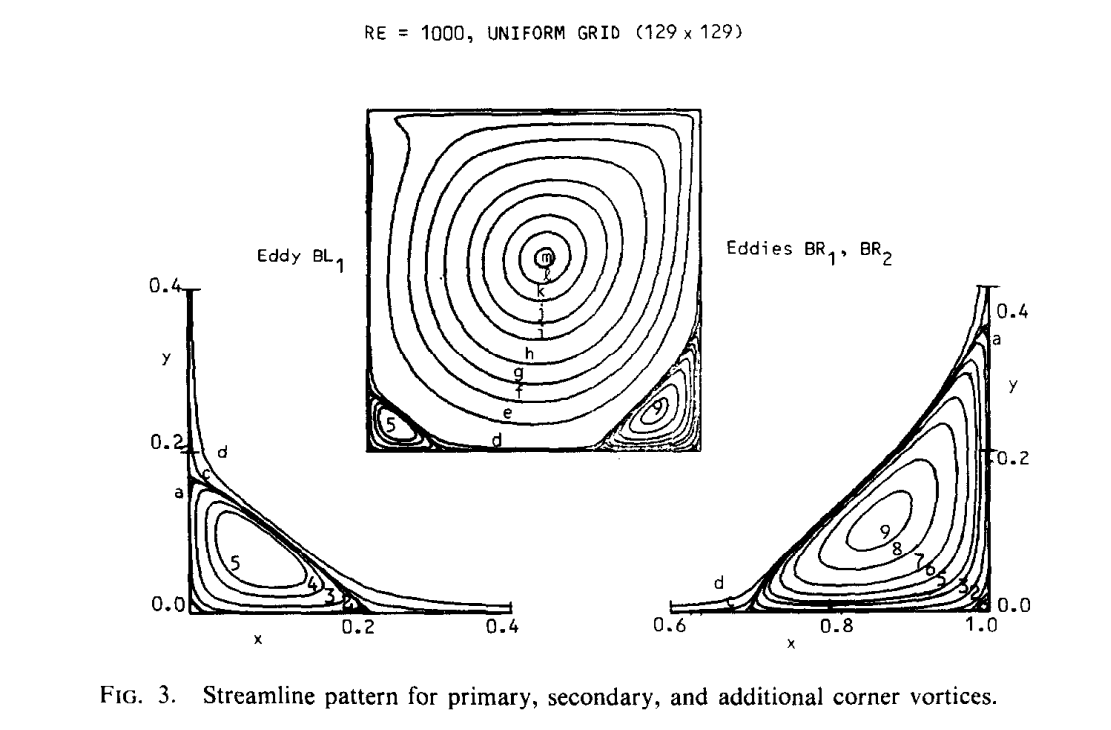
\includegraphics[width=.9\textwidth]{./img/ghia_solution_Re1000}
    \caption{Solution from Ghia et al. \cite{Ghia1982HighReSF} for the lid-driven cavity flow at $Re = 1000$.}
    \label{fig:ghia_solution_Re1000}
\end{figure}

After running the \acrshort{scgs} algorithm, we obtained the solution reported in Figure \ref{fig:scgs_solution_Re1000}.

\begin{figure}[H]
    \centering
    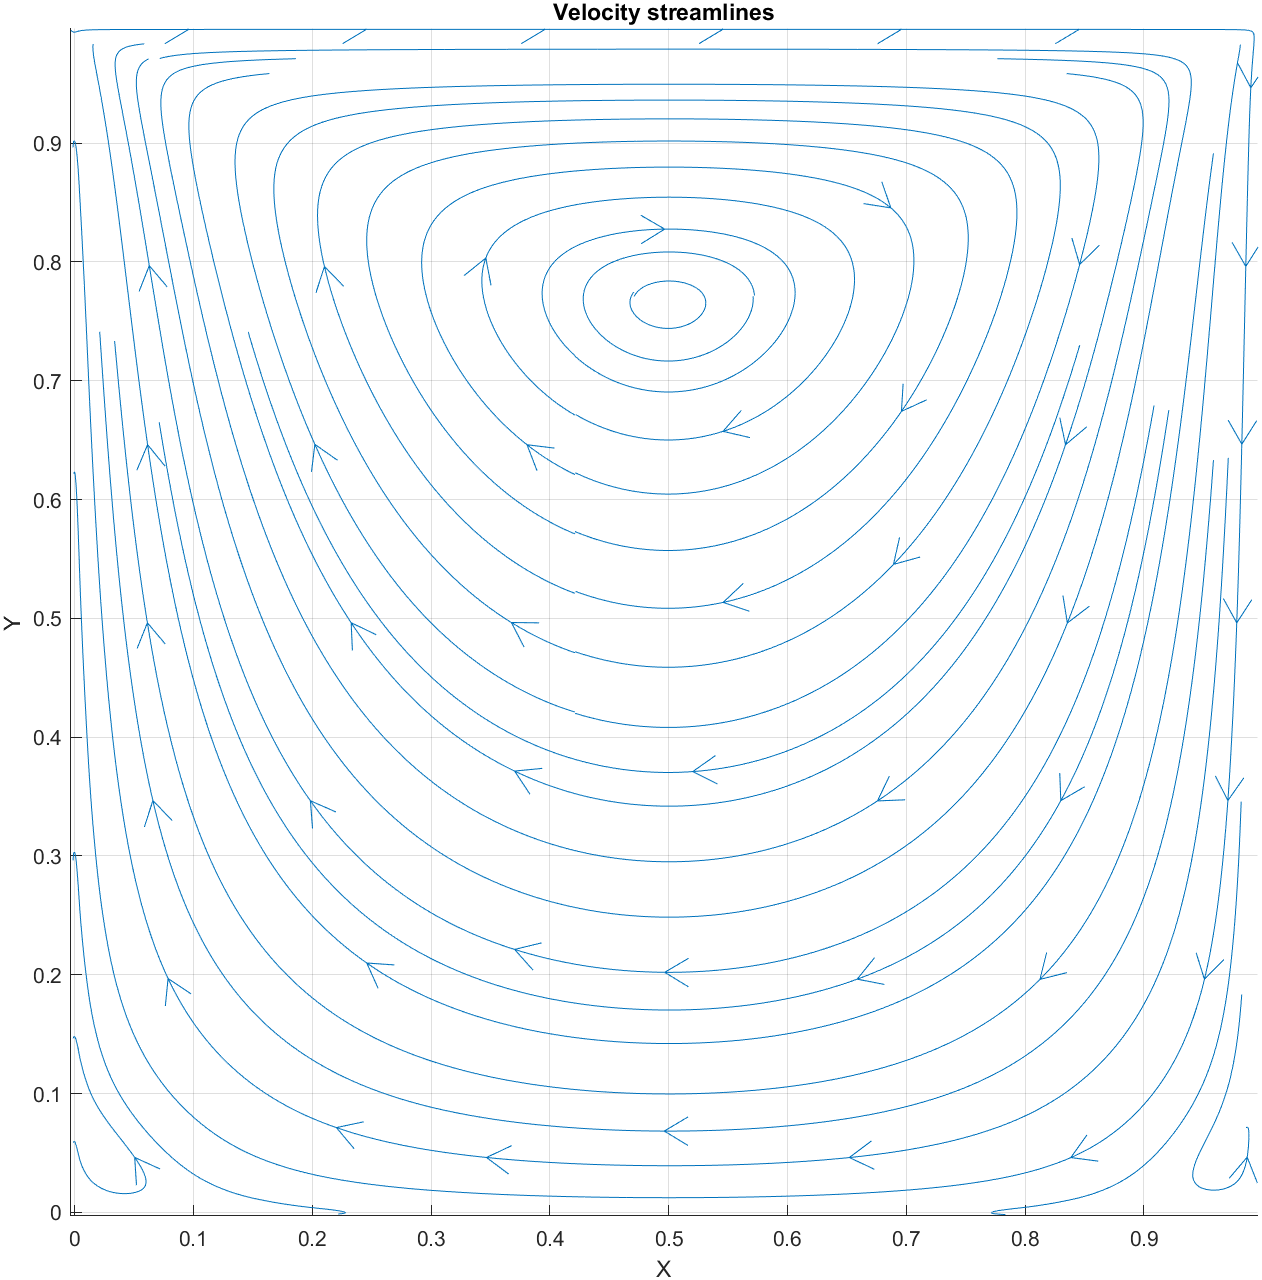
\includegraphics[width=.6\textwidth]{./img/scgs_solution_Re1000}
    \caption{Solution obtained using the \acrshort{scgs} algorithm for the lid-driven cavity flow at $Re = 1000$.}
    \label{fig:scgs_solution_Re1000}
\end{figure}

As it is easy to observe from the streamline plots, the solution obtained using our code is not in agreement with the one reported by Ghia.

In particular, the eddies at the bottom corners of the cavity are not present in our solution, and the overall distribution of the streamlines is basically symmetrical which intuitively is not correct.

Similar considerations can be made by comparing numerically the velocity profiles between the two solutions.

From Figure \ref{fig:velocity_profiles_Re1000_comparison} it's clearly visible how the two solutions are not in agreement.

\begin{figure}[H]
    \begin{minipage}[b]{0.45\textwidth}
        \centering
        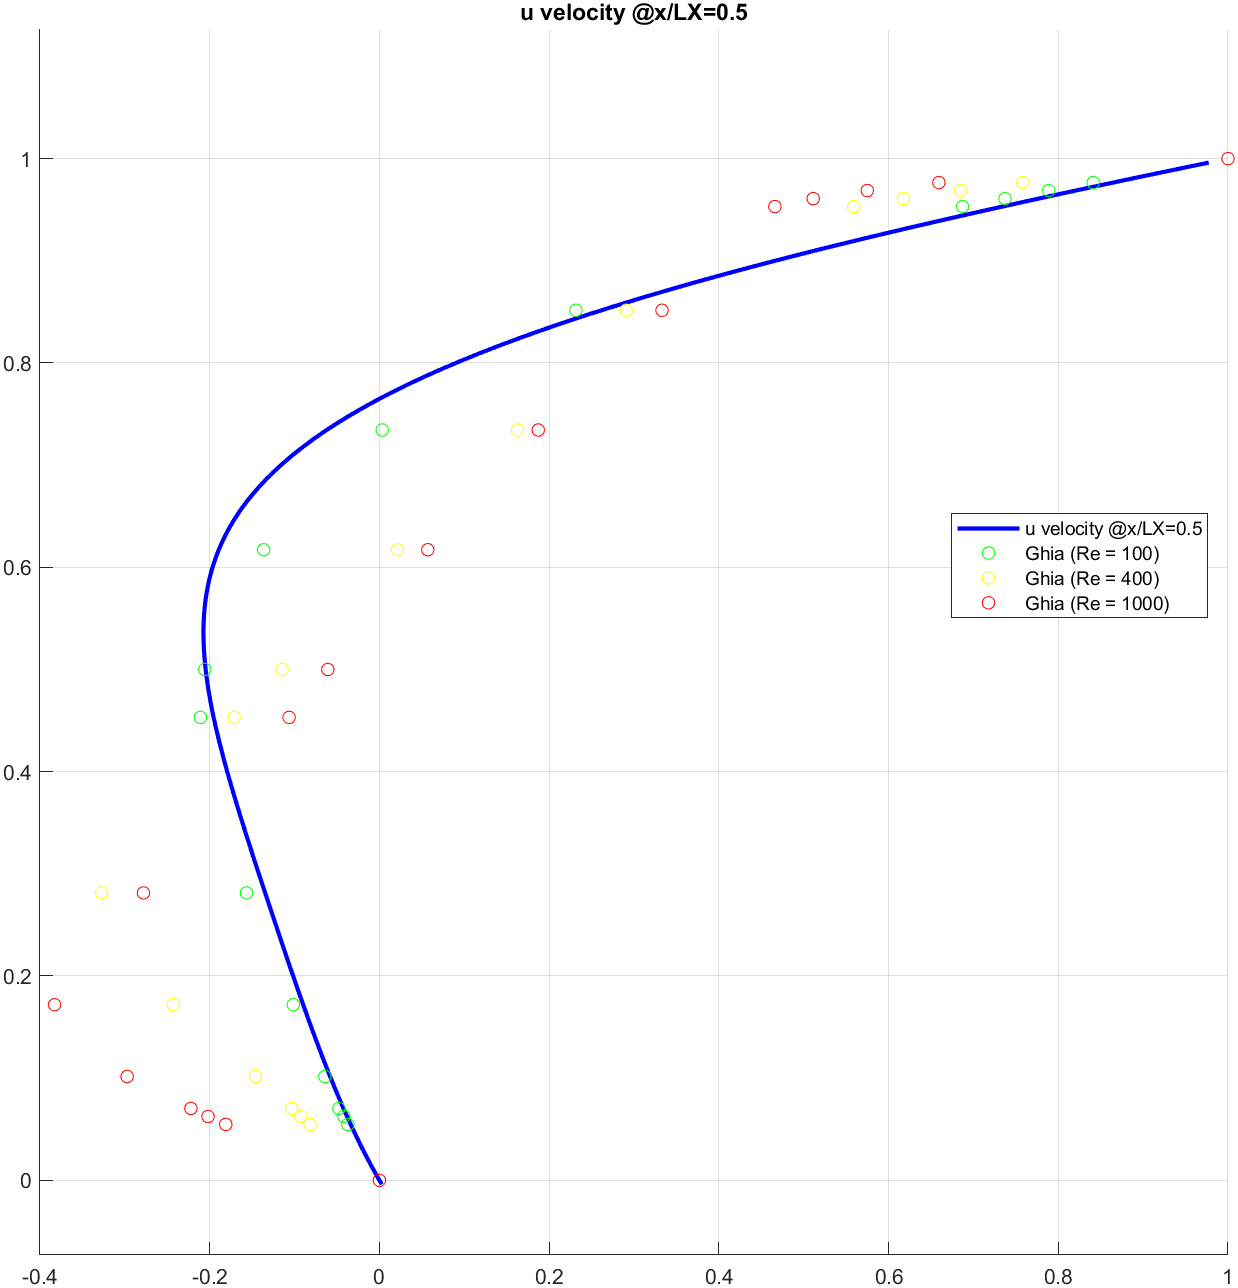
\includegraphics[width=.9\textwidth]{./img/velocity_profiles_Re1000_u}
        \caption{$u(y) @ x/L_x = 0.5$}
        \label{fig:velocity_profiles_Re1000_u}
    \end{minipage}
    \hfill
    \begin{minipage}[b]{0.45\textwidth}
        \centering
        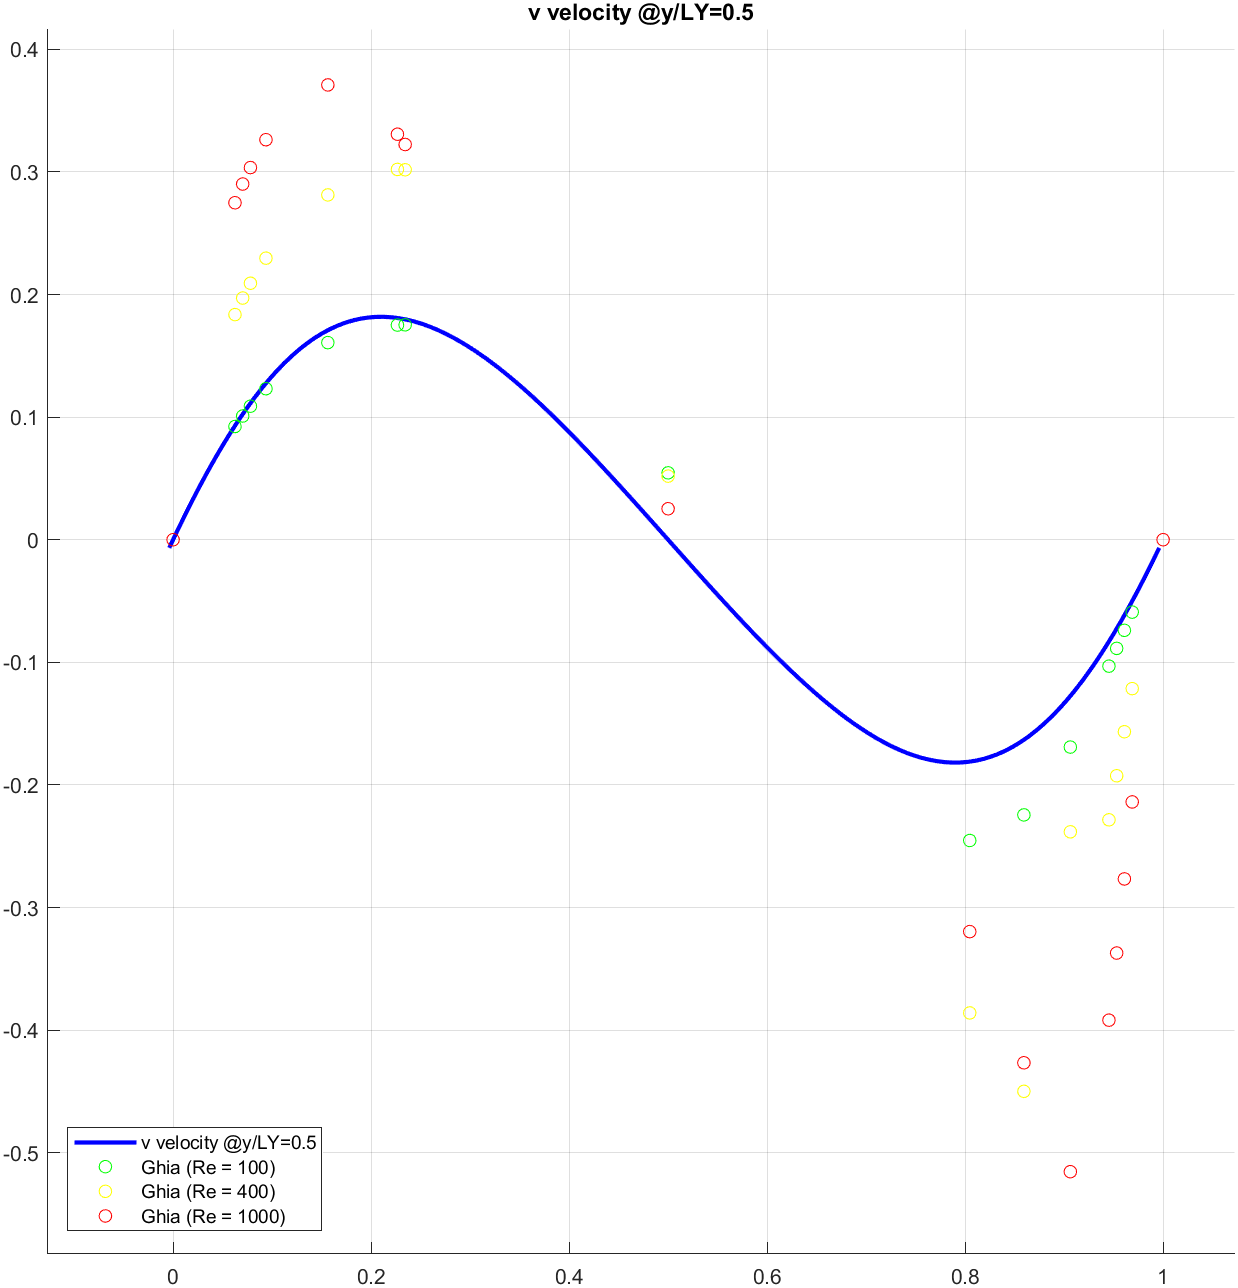
\includegraphics[width=.9\textwidth]{./img/velocity_profiles_Re1000_v}
        \caption{$v(x) @ y/L_y = 0.5$}
        \label{fig:velocity_profiles_Re1000_v}
    \end{minipage}
    \caption{Comparison of the velocity profiles.}
    \label{fig:velocity_profiles_Re1000_comparison}
\end{figure}

We also have tried to run the code with different parameters, but the results are always not in agreement with the ones reported by Ghia et al. \cite{Ghia1982HighReSF}.

\paragraph{Note}

We will try to fix the bug and update the results as soon as possible.
Not for the assegnment or the mark related to it, but for the sake of the project itself (it's useless to have a code that doesn't work as expected\dots).


\clearpage
\bibliographystyle{plain}
\bibliography{ref}

\clearpage
\appendix
\label{sec:appendix}

\section{Mathematica code}

Here follows the \texttt{Mathematica} notebook used for symbolic analysis of the discretized schemes.

\lstinputlisting[
    style=mathematica,
    language=Mathematica,
    caption=Mathematica notebook used for symbolic analysis of the discretized schemes.,
]{files/Mathematica.txt}


\clearpage
\section{C code}
The complete codebase is available on GitHub at \url{https://github.com/Bocchio01/CFD_Simulation_Engine}, along with its technical documentation.

\lstinputlisting[
    style=C,
    language=C,
    caption=SCGS Core algorithm implementation in C.,
]{files/SCGS.c}

\lstinputlisting[
    style=C,
    language=C,
    caption=SCGS Boundary Conditions implementation in C.,
]{files/SCGSBC.c}

\lstinputlisting[
    style=C,
    language=C,
    caption=Convection Schemes implementation in C.,
]{files/convection.c}

\lstinputlisting[
    style=C,
    language=C,
    caption=Diffusion Schemes implementation in C.,
]{files/diffusion.c}

\end{document}
